\documentclass[dvipsnames]{beamer} % Use handout option to remove pauses.
\usetheme{default}
\usefonttheme{structurebold}
\usefonttheme[onlymath]{serif}
\usepackage[UKenglish,cleanlook]{isodate}                                  % Set default date and date display
\usepackage[T1]{fontenc}
% Slide title background color
\definecolor{background}{HTML}{ede6d8}
% Slide title text color
\definecolor{titleText}{HTML}{B40404}
% Add slide numbers in bottom right corner
\defbeamertemplate{headline}{my header}{
    \vskip1pt
    \makebox[0pt][l]{\,\insertsection}
    \hspace*{\fill}\insertshorttitle\hspace*{\fill}
    \llap{\insertframenumber\,/\,\inserttotalframenumber\,}
}
\setbeamertemplate{headline}[my header]
% Add name at the bottom
\setbeamercolor{footlinecolor}{fg=black,bg=background}
\defbeamertemplate{footline}{my footer}{%
    \begin{beamercolorbox}[wd=\paperwidth,leftskip=0.25cm,rightskip=0.25cm]{footlinecolor}
    \hfill
    \insertshortauthor
    \end{beamercolorbox}
}
\setbeamertemplate{footline}[my footer]
\setbeamertemplate{navigation symbols}[default]
\usepackage{graphicx}
% Set font sizes for frame title and subtitle
\setbeamerfont{frametitle}{size=\fontsize{15}{16}}
\setbeamerfont{framesubtitle}{size=\small}
% Set left and right text margins
\setbeamersize{text margin left=5mm, text margin right=5mm}
\usepackage{booktabs,multirow}
\usepackage{subcaption}   % Sub figures.
\usepackage{tikz}
\usetikzlibrary{shapes,decorations,decorations.pathreplacing,arrows,calc,arrows.meta,fit,positioning}
\tikzset{
    auto,node distance =1 cm and 1 cm,semithick,
    state/.style ={ellipse, draw, minimum width = 0.7 cm},
    point/.style = {circle, draw, inner sep=0.04cm,fill,node contents={}},
    bidirected/.style={Latex-Latex,dashed},
    el/.style = {inner sep=2pt, align=left, sloped}
}
\usepackage{mathtools}                                                     % Various maths functions
\usepackage{amssymb}                                                       % Various maths functions
\usepackage{amsmath}                                                       % Various maths functions
\usepackage{dsfont}                                                        % Various maths functions
\usepackage{centernot}                                                     % center \not usage
\usepackage{siunitx} \sisetup{round-mode=places, round-precision=3}        % Formalise use of units and numbers among text
\usepackage[normalem]{ulem} % Strike-through package
\renewcommand{\vec}[1]{\boldsymbol{\mathit{#1}}}                           % vector notation shortcut
\newcommand{\mat}[1]{\boldsymbol{\mathit{#1}}}                             % matrix notation shortcut
\DeclarePairedDelimiter\abs{\lvert}{\rvert}                                % absolute value notation shortcut
\DeclarePairedDelimiter\norm{\lVert}{\rVert}                               % norm notation shortcut
\newcommand{\Prob}[1]{\Pr\left( #1 \right)}                         % SHortcut for probability notation
\newcommand{\Probgiven}[2]{\Pr\left( #1 \, \middle\vert \, #2 \right)} % SHortcut for probability notation, given
\newcommand{\E}[2][]{\mathbb{E}_{#1} \left[ #2 \right]}                    % Expectation (with optional subscript) shortcut
\newcommand{\Egiven}[3][]{\mathbb{E}_{#1} \left[ #2 \, \middle\vert \, #3 \right]} % Expectation given (with optional subscript) shortcut
\newcommand{\Var}[2][]{\text{Var}_{#1} \left( #2 \right)}                  % Variation (with optional subscript) shortcut
\newcommand{\Cov}[1]{\text{Cov} \left( #1 \right)}                         % Covariance (with optional subscript) shortcut
\newcommand{\indicator}[1]{\mathds{1}\left\{ #1 \right\}}                  % SHortcut for indicator function
\newcommand{\indep}{\, \raisebox{0.05em}{\rotatebox[origin=c]{90}{$\models$}} \,}% Statistical independence symbol.
\newcommand{\diff}[2][]{\frac{d#1}{d#2}}                                   % SHortcut for differential fraction as a function
\newcommand{\partialdiff}[2][]{\frac{\partial#1}{\partial#2}}              % SHortcut for partial differential fraction as a function
\renewcommand{\hat}[1]{\widehat{#1}}                                       % Default estimator notation is widehat
\renewcommand{\bar}[1]{\overline{#1}}                                      % Make over bar look nicer
\renewcommand{\tilde}[1]{\widetilde{#1}}                                   % Make over tilde look better
% Citations
\usepackage{natbib}                                        % Citation package, see https://en.wikibooks.org/wiki/LaTeX/Bibliography_Management#Natbib
\usepackage{hyperref}                                        % Allow for links across the text, with colour options
\usepackage{setspace}
\settowidth{\leftmargini}{\usebeamertemplate{itemize item}}
\addtolength{\leftmargini}{\labelsep}
\usepackage{soul,color,xcolor} % Text highlighting
\newcommand{\eqhighlight}[2]{\colorbox{#1!50}{$\displaystyle#2$}}
\makeatletter
\let\HL\hl
\renewcommand\hl{%
    \let\set@color\beamerorig@set@color
    \let\reset@color\beamerorig@reset@color
    \HL}
\makeatother
\newcommand{\mathcolorbox}[2]{\colorbox{#1}{$\displaystyle #2$}}
% Set colors
\setbeamercolor{block title}{use=structure,fg=white,bg=structure.fg!75!black}
\setbeamercolor{block body}{parent=normal text,use=block title,bg=block title.bg!10!bg}
\setbeamercovered{transparent}
\setbeamercolor{postit}{fg=black, bg=yellow}
\setbeamercolor{frametitle}{bg=background, fg=titleText}
\setbeamercolor{subtitle}{fg=titleText}
% Command to align text
\renewcommand{\raggedright}{\leftskip=0pt \rightskip=0pt plus 0cm}
% Remove the useless buttons.
\setbeamertemplate{navigation symbols}{}
\useoutertheme[footline=empty,subsection=false]{miniframes}
\useinnertheme{circles}

%-------------------------------------------------------------------------------
% Title Page
%-------------------------------------------------------------------------------
\title{\color{titleText}
    Causal Mediation in Natural Experiments
}
\author[Senan Hogan-Hennessy, Cornell University]{
    Senan Hogan-Hennessy \\
    Economics Department, Cornell University \\ %\vspace{0.5cm}
    \href{mailto:seh325@cornell.edu}{\textcolor{blue}{seh325@cornell.edu}}
}
\date{} % Date, can be changed to a custom date

%-------------------------------------------------------------------------------
% Opening Slides
\begin{document}
% Justify text through-out.
\raggedright
%-------------------------------------------------------------------------------
%% Title page
\begin{frame}[noframenumbering, plain]
    % Print the title page as the first slide
    \titlepage
    \vspace{-1.5cm}
    \begin{center}
        
\includegraphics[width=2cm]{presentation-files/cornell}

        \vspace{0.5cm}
        Econometric Society World Congress, Seoul \\
        22 August 2025
        %Meeting of the European Economic Association \\
        %Bordeaux Sciences \'Economiques \\
        %25 August 2025
    \end{center}
\end{frame}

%-------------------------------------------------------------------------------
% Introduction.
\section{Introduction}
%-------------------------------------------------------------------------------
\begin{frame}
    \frametitle{Oregon Health Insurance Experiment}
    Oregon gave health insurance by wait-list lottery (Finkelstein et al, 2012).
    \vspace{-0.35cm}
    \begin{figure}
        \centering
        \singlespacing
        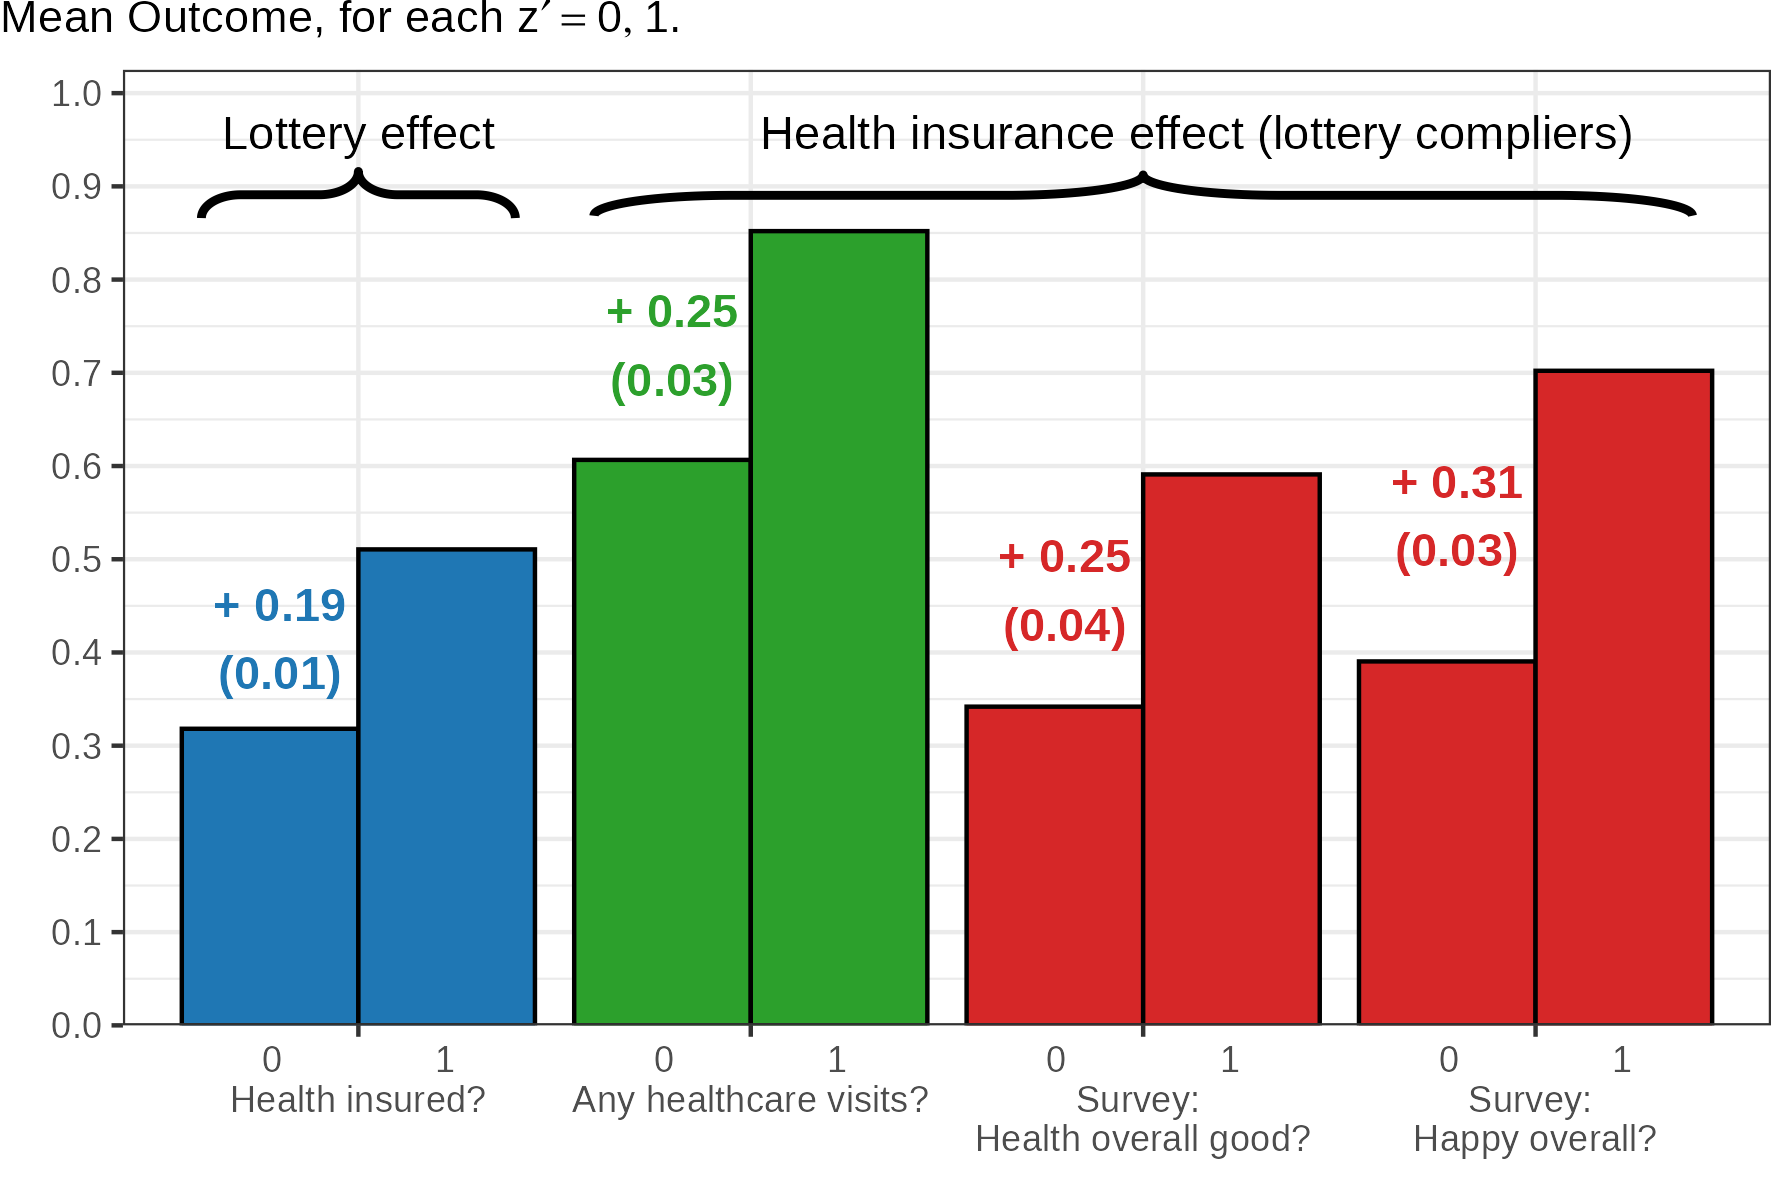
\includegraphics[width=0.85\textwidth]{
            ../text/sections/figures/insurance-effects.png}
    \end{figure}
\end{frame}
%-------------------------------------------------------------------------------
\begin{frame}[noframenumbering]
    \frametitle{Oregon Health Insurance Experiment}
    Oregon gave health insurance by wait-list lottery (Finkelstein et al, 2012).
    \vspace{-0.25cm}
    \begin{figure}
        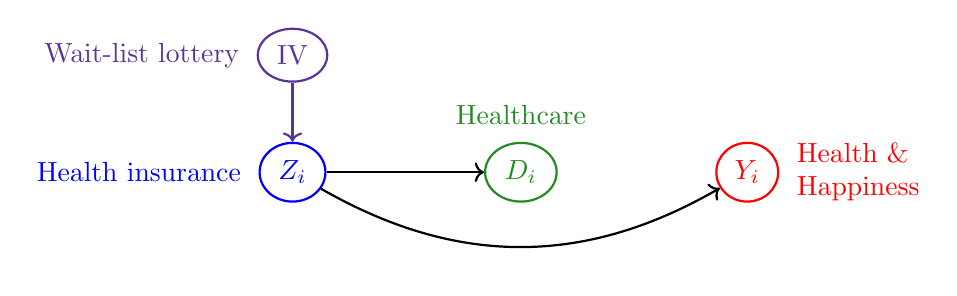
\begin{tikzpicture}
            \node[state,thick,ForestGreen] (mediator) at (0,0) {$D_i$};
            \node[state,thick,blue] (treatment) [left=2cm of mediator] {$Z_i$};
            \node[state,thick,red] (outcome)   [right=2cm of mediator] {$Y_i$};
            % Label Z_i, D, Y_i
            \node[color=ForestGreen] [above=0.1cm of mediator] {Healthcare};
            \node[color=blue] [left=0.1cm of treatment] {Health insurance};
            \node[color=red,align=left] [right=0.1cm of outcome] {Health \& \\ Happiness};
            % Draw the causal arrows
            \path[->, thick] (treatment) edge (mediator);
            %\path[->, dashed,color=gray] (mediator) edge (outcome);
            \path[->, thick] (treatment) edge[bend right=30] (outcome);
            % Label the IV.
            \node[state,thick,RoyalPurple] (treatmentIV) [above=0.75cm of treatment] {IV};
            \node[color=RoyalPurple] [left=0.1cm of treatmentIV] {Wait-list lottery};
            \path[->,thick,color=RoyalPurple] (treatmentIV) edge (treatment);
        \end{tikzpicture}
    \end{figure}
    $\Rightarrow$ suggestive evidence of healthcare visits as a mechanism for health insurance gains.
    \begin{itemize}
        \item Missing the $D_i \to Y_i$ edge of the triangular system...
        \item Is it small, large, or even existent?
        \item Where else do we accept assumed causal effects without evidence?
    \end{itemize}
\end{frame}
%-------------------------------------------------------------------------------
\begin{frame}
    \frametitle{Oregon Health Insurance Experiment}
    Oregon gave health insurance by wait-list lottery (Finkelstein et al, 2012).
    \vspace{-0.25cm}
    \begin{figure}
        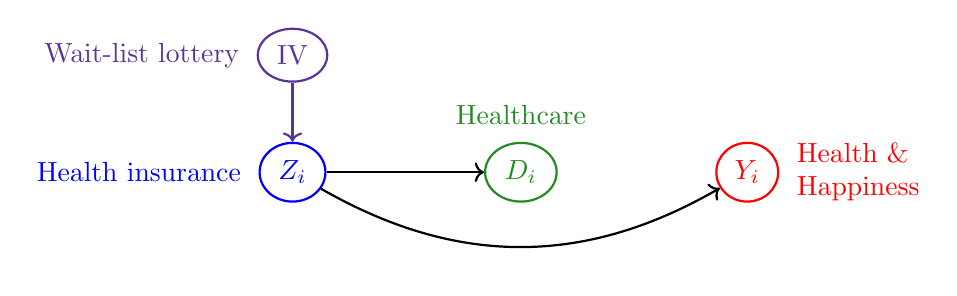
\begin{tikzpicture}
            \node[state,thick,ForestGreen] (mediator) at (0,0) {$D_i$};
            \node[state,thick,blue] (treatment) [left=2cm of mediator] {$Z_i$};
            \node[state,thick,red] (outcome)   [right=2cm of mediator] {$Y_i$};
            % Label Z_i, D, Y_i
            \node[color=ForestGreen] [above=0.1cm of mediator] {Healthcare};
            \node[color=blue] [left=0.1cm of treatment] {Health insurance};
            \node[color=red,align=left] [right=0.1cm of outcome] {Health \& \\ Happiness};
            % Draw the causal arrows
            \path[->, thick] (treatment) edge (mediator);
            %\path[->, dashed,color=gray] (mediator) edge (outcome);
            \path[->, thick] (treatment) edge[bend right=30] (outcome);
            % Label the IV.
            \node[state,thick,RoyalPurple] (treatmentIV) [above=0.75cm of treatment] {IV};
            \node[color=RoyalPurple] [left=0.1cm of treatmentIV] {Wait-list lottery};
            \path[->,thick,color=RoyalPurple] (treatmentIV) edge (treatment);
        \end{tikzpicture}
    \end{figure}
    $\Rightarrow$ suggestive evidence of healthcare visits as a mechanism for health insurance gains.
    \begin{enumerate}
        \item This paper considers an alternative approach, Causal Mediation (CM)
        \item CM explicitly states its estimands $+$ identifying assumptions
        \item Hugely popular in other fields, but not so in quas-experimental economics (for good reason...) 
    \end{enumerate}
\end{frame}
%-------------------------------------------------------------------------------
\begin{frame}
    \frametitle{Introduction}
    This project examines Causal Mediation (CM) with economic perspective:
    \begin{enumerate}
        \item Problems with conventional approach to CM (and informal mechanism analyses) in social science settings --- focusing on natural experiments.
        \\ \textbf{[Negative result]}
        \item Recovering valid CM effects under selection-into-mediator, with modelling asumptions.
        \\ \textbf{[Positive result]}
    \end{enumerate}
    \par\noindent\rule{\textwidth}{0.4pt}
    Brings together ideas from two different literatures:
    \begin{itemize}
        \item \textbf{Causal Mediation (CM).}
        \\ Imai Keele Yamamoto (2010), Fr\"olich Huber (2017), Deuchert Huber Schelker (2019), Huber (2020), Kwon Roth (2024).
        \item \textbf{Labour theory, Selection-into-treatment, MTEs.}
        \\ Roy (1951), Heckman (1979), Heckman Honor\'e (1990), Vycatil (2002), Heckman Vycatil (2005), Kline Walters (2019).
    \end{itemize}
\end{frame}%-------------------------------------------------------------------------------
\section{1. CM}
%-------------------------------------------------------------------------------
\begin{frame}
    \frametitle{Direct \& Indirect Effects --- Model}
    Consider binary \textcolor{blue}{treatment $Z_i = 0, 1$},
    binary \textcolor{ForestGreen}{mediator $D_i = 0, 1$},
    and continuous \textcolor{red}{outcome $Y_i$} for individuals $i = 1, \hdots, N$.
    \vskip-0.5cm
    \begin{figure}
        \centering
        \singlespacing
        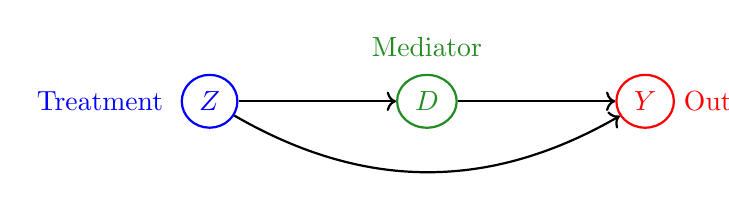
\begin{tikzpicture}
            \node[state, thick,ForestGreen] (mediator) at (0,0) {$D$};
            \node[state, thick,blue] (treatment) [left=2cm of mediator] {$Z$};
            \node[state, thick,red] (outcome) [right=2cm of mediator] {$Y$};
            % Label Z, D, Y
            \node[color=ForestGreen] [above=0.1cm of mediator] {Mediator};
            \node[color=blue] [left=0.1cm of treatment] {Treatment};
            \node[text width=0.1cm, color=red] [right=-0.01cm of outcome] {Outcome};
            % Draw the causal arrows
            \path[->, thick] (treatment) edge (mediator);
            \path[->, thick] (mediator) edge (outcome);
            \path[->, thick] (treatment) edge[bend right=30] (outcome);
            % Label direct and indirect effect
            %\node[color=orange] [above left=-0.35cm and 0.2cm of mediator] {First-stage};
            %\node[color=orange] [above right=-0.3cm and 0.4cm of mediator] {Indirect};
            %\node[color=orange] [below=0.5cm of mediator] {Direct Effect};
        \end{tikzpicture}
    \end{figure}
    \vskip-0.25cm
    \par\noindent\rule{\textwidth}{0.4pt}
    \begin{align*}
        & \textcolor{ForestGreen}{\text{Mediator }D_i} \text{ is a function of } \textcolor{blue}{Z_i}.
        & \textcolor{red}{\text{Outcome }Y_i} \text{ is a function of both }
        \textcolor{blue}{Z_i}, \textcolor{ForestGreen}{D_i}. \\
        & D_i = \begin{cases}
            D_i(0), \text{ if } Z_i = 0 \\
            D_i(1), \text{ if } Z_i = 1.
        \end{cases}
        & Y_i = \begin{cases}
            Y_i(0, D_i(0)), \text{ if } Z_i = 0 \\
            Y_i(1, D_i(1)), \text{ if } Z_i = 1.
        \end{cases}
    \end{align*}
\end{frame}
%-------------------------------------------------------------------------------
\begin{frame}[noframenumbering]
    \frametitle{Direct \& Indirect Effects --- Model}
    Consider binary \textcolor{blue}{treatment $Z_i = 0, 1$},
    binary \textcolor{ForestGreen}{mediator $D_i = 0, 1$},
    and continuous \textcolor{red}{outcome $Y_i$} for individuals $i = 1, \hdots, N$.
    \vskip-0.5cm
    \begin{figure}
        \centering
        \singlespacing
        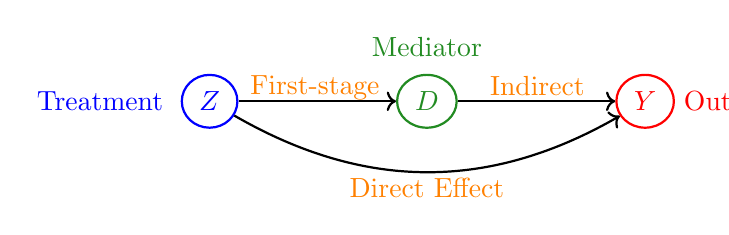
\begin{tikzpicture}
            \node[state, thick,ForestGreen] (mediator) at (0,0) {$D$};
            \node[state, thick,blue] (treatment) [left=2cm of mediator] {$Z$};
            \node[state, thick,red] (outcome) [right=2cm of mediator] {$Y$};
            % Label Z, D, Y
            \node[color=ForestGreen] [above=0.1cm of mediator] {Mediator};
            \node[color=blue] [left=0.1cm of treatment] {Treatment};
            \node[text width=0.1cm, color=red] [right=-0.01cm of outcome] {Outcome};
            % Draw the causal arrows
            \path[->, thick] (treatment) edge (mediator);
            \path[->, thick] (mediator) edge (outcome);
            \path[->, thick] (treatment) edge[bend right=30] (outcome);
            % Label direct and indirect effect
            \node[color=orange] [above left=-0.35cm and 0.2cm of mediator] {First-stage};
            \node[color=orange] [above right=-0.3cm and 0.4cm of mediator] {Indirect};
            \node[color=orange] [below=0.5cm of mediator] {Direct Effect};
        \end{tikzpicture}
    \end{figure}
    \par\noindent\rule{\textwidth}{0.4pt}
    Suppose $Z_i$ is ignorable, conditional on $\vec X_i$.
    \[ Z_i \indep  D_i(z), Y_i(z', d') \; \; | \;\; \vec X_i \text{ for } z, z', d' = 0, 1. \]

    Only two causal effects are identified so far.
    \begin{align*}
    \text{ATE:} \;\; \E{Y_i(1, D_i(1)) - Y_i(0, D_i(0))}
        &= \Egiven{Y_i}{Z_i = 1} - \Egiven{Y_i}{Z_i = 0} \\
    \text{Average first-stage:} \;\; \E{D_i(1) - D_i(0)}
        &=\Egiven{D_i}{Z_i = 1} - \Egiven{D_i}{Z_i = 0}
    \end{align*}
\end{frame}
%-------------------------------------------------------------------------------
\begin{frame}[noframenumbering]
    \frametitle{Direct \& Indirect Effects --- Model}
    Consider binary \textcolor{blue}{treatment $Z_i = 0, 1$},
    binary \textcolor{ForestGreen}{mediator $D_i = 0, 1$},
    and continuous \textcolor{red}{outcome $Y_i$} for individuals $i = 1, \hdots, N$.
    \vskip-0.5cm
    \begin{figure}
        \centering
        \singlespacing
        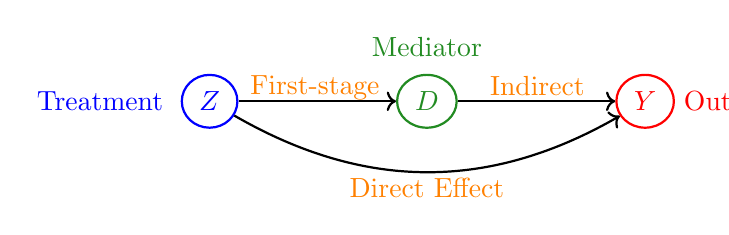
\begin{tikzpicture}
            \node[state, thick,ForestGreen] (mediator) at (0,0) {$D$};
            \node[state, thick,blue] (treatment) [left=2cm of mediator] {$Z$};
            \node[state, thick,red] (outcome) [right=2cm of mediator] {$Y$};
            % Label Z, D, Y
            \node[color=ForestGreen] [above=0.1cm of mediator] {Mediator};
            \node[color=blue] [left=0.1cm of treatment] {Treatment};
            \node[text width=0.1cm, color=red] [right=-0.01cm of outcome] {Outcome};
            % Draw the causal arrows
            \path[->, thick] (treatment) edge (mediator);
            \path[->, thick] (mediator) edge (outcome);
            \path[->, thick] (treatment) edge[bend right=30] (outcome);
            % Label direct and indirect effect
            \node[color=orange] [above left=-0.35cm and 0.2cm of mediator] {First-stage};
            \node[color=orange] [above right=-0.3cm and 0.4cm of mediator] {Indirect};
            \node[color=orange] [below=0.5cm of mediator] {Direct Effect};
        \end{tikzpicture}
    \end{figure}
    \vskip-0.5cm
    \par\noindent\rule{\textwidth}{0.4pt}
    First-stage and ATE answer important questions:
    \begin{itemize}
        \item Did socialised health insurance increase healthcare use, and improve health? (Finkelstein et al, 2012).
    \end{itemize}
    Unanswered questions about the mechanism(s):
    \begin{itemize}
        \item Did health benefits come from using health care more?
        Health gains from reduced uncertainty --- i.e., insurance?
        \item Is health insurance more about the health or more about the insurance?
    \end{itemize}
\end{frame}%-------------------------------------------------------------------------------
\begin{frame}[noframenumbering]
    \frametitle{Direct \& Indirect Effects --- Model}
    Consider binary \textcolor{blue}{treatment $Z_i = 0, 1$},
    binary \textcolor{ForestGreen}{mediator $D_i = 0, 1$},
    and continuous \textcolor{red}{outcome $Y_i$} for individuals $i = 1, \hdots, N$.
    \vskip-0.5cm
    \begin{figure}
        \centering
        \singlespacing
        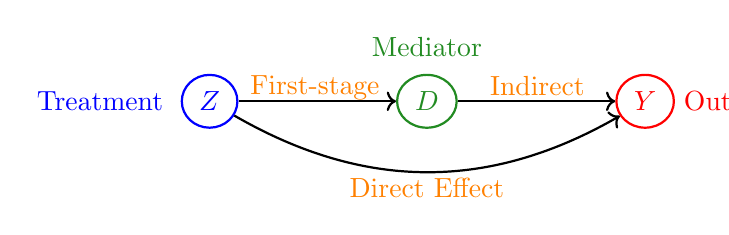
\begin{tikzpicture}
            \node[state, thick,ForestGreen] (mediator) at (0,0) {$D$};
            \node[state, thick,blue] (treatment) [left=2cm of mediator] {$Z$};
            \node[state, thick,red] (outcome) [right=2cm of mediator] {$Y$};
            % Label Z, D, Y
            \node[color=ForestGreen] [above=0.1cm of mediator] {Mediator};
            \node[color=blue] [left=0.1cm of treatment] {Treatment};
            \node[text width=0.1cm, color=red] [right=-0.01cm of outcome] {Outcome};
            % Draw the causal arrows
            \path[->, thick] (treatment) edge (mediator);
            \path[->, thick] (mediator) edge (outcome);
            \path[->, thick] (treatment) edge[bend right=30] (outcome);
            % Label direct and indirect effect
            \node[color=orange] [above left=-0.35cm and 0.2cm of mediator] {First-stage};
            \node[color=orange] [above right=-0.3cm and 0.4cm of mediator] {Indirect};
            \node[color=orange] [below=0.5cm of mediator] {Direct Effect};
        \end{tikzpicture}
    \end{figure}
    \vskip-0.5cm
    \par\noindent\rule{\textwidth}{0.4pt}
    \[ \text{Average Direct Effect (ADE)}: \;\;\;
        \E{Y_i\left(\eqhighlight{blue}{1}, D_i(Z_i) \right)
            - Y_i\left(\eqhighlight{blue}{0}, D_i(Z_i) \right)} \]
    \vskip-0.35cm
    \begin{itemize}
        \item ADE is causal effect $Z\to Y$, blocking the indirect $D$ path.
    \end{itemize}
    \vskip0.25cm
    \[ \text{Average Indirect Effect (AIE):} \;\;\;
    \E{Y_i\left(Z_i, \eqhighlight{ForestGreen}{D_i(1)} \right)
        - Y_i\left(Z_i, \eqhighlight{ForestGreen}{D_i(0)} \right)} \]
    \vskip-0.25cm
    \begin{itemize}
        \item AIE is causal effect of $D(Z) \to Y$, blocking the direct $Z$ path.\footnote[frame]{
            Note: AIE $=$ fraction of $D(Z)$ compliers $\times$ average effect $D\to Y$ among compliers.}
    \end{itemize}
\end{frame}
%-------------------------------------------------------------------------------
\begin{frame}
    \frametitle{Direct \& Indirect Effects --- Identification} 
    \textbf{Sequential ignorability} (\textbf{SI}, Imai Keele Yamamoto 2010):
    \vskip0.125cm
    Assume \textcolor{ForestGreen}{mediator $D_i$} is \textit{also} ignorable, conditional on $\vec X_i$ and \textcolor{blue}{$Z_i$ realisation}
    \[ D_i \indep Y_i(z', d') \;\; | \;\; \vec X_i, Z_i = z',
        \text{ for } z', d' = 0, 1. \]
    \vskip-0.25cm
    \par\noindent\rule{\textwidth}{0.4pt}
    If \textbf{SI} holds then ADE and AIE are identified by two-stage regression:
    \makebox[\textwidth]{\parbox{1.25\textwidth}{
        \footnotesize
\[ \E[D_i, \vec X_i]{
    \underbrace{\Egiven{Y_i}{Z_i = 1, D_i, \vec X_i} - \Egiven{Y_i}{Z_i = 0, D_i, \vec X_i}}_{\text{Second-stage regression, $Y_i$ on $Z_i$ holding $D_i, \vec X_i$ constant}}}
    = \text{ADE} \]
\[ \E[Z_i, \vec X_i]{ \begin{aligned}&\underbrace{\Big(
    \Egiven{D_i}{Z_i = 1, \vec X_i} - \Egiven{D_i}{Z_i = 0, \vec X_i} \Big)}_{\text{First-stage regression, $D_i$ on $Z_i$}}\\
    &\times \underbrace{\Big(
    \Egiven{Y_i}{Z_i, D_i = 1, \vec X_i} - \Egiven{Y_i}{Z_i, D_i = 0, \vec X_i} \Big)}_{\text{Second-stage regression, $Y_i$ on $D_i$ holding $Z_i, \vec X_i$ constant}} \end{aligned}} = \text{AIE} \]
}}
\end{frame}
%-------------------------------------------------------------------------------
\begin{frame}[noframenumbering]
    \frametitle{Direct \& Indirect Effects --- Identification} 
    \textbf{Sequential ignorability} (\textbf{SI}, Imai Keele Yamamoto 2010):
    \vskip0.125cm
    Assume \textcolor{ForestGreen}{mediator $D_i$} is \textit{also} ignorable, conditional on $\vec X_i$ and \textcolor{blue}{$Z_i$ realisation}
    \[ D_i \indep Y_i(z', d') \;\; | \;\; \vec X_i, Z_i = z',
    \text{ for } z', d' = 0, 1. \]
    \par\noindent\rule{\textwidth}{0.4pt}
    E.g., OLS simultaneous regression (Imai Keele Yamamoto, 2010):
    \begin{align*}
        &\textcolor{blue}{Z_i \leftarrow \text{ Treatment}} &
        \text{First-stage: }
            \textcolor{ForestGreen}{D_i}
                &= \phi + \pi \textcolor{blue}{Z_i} + \vec \psi_1' \vec X_i + U_i \\
        &\textcolor{ForestGreen}{D_i \leftarrow \text{ Mediator}} &
        \text{Second-stage: }
            \textcolor{red}{Y_i}
                &= \alpha
                    + \beta \textcolor{ForestGreen}{D_i}
                    + \gamma \textcolor{blue}{Z_i}
                    + \delta \textcolor{blue}{Z_i} \textcolor{ForestGreen}{D_i}
                    + \vec \psi_2' \vec X_i
                    + \varepsilon_i \\
        &\textcolor{red}{Y_i \leftarrow \text{ Outcome}} &
            \implies \textcolor{Orange}{\text{ADE }}
            &= \gamma + \delta \E{\textcolor{ForestGreen}{D_i}} \\
        &   &\textcolor{Orange}{\text{AIE }}
            &= \pi \left( \beta + \delta \E{\textcolor{blue}{Z_i}} \right)
    \end{align*}
    i.e., a regression decomposition.

    \vfill
    Other estimation methods do the same decomposition, avoiding linearity assumptions (see Huber 2020 for an overview).
\end{frame}
%-------------------------------------------------------------------------------
\begin{frame}
    \frametitle{Direct \& Indirect Effects --- Selection} 
    $\implies$ Great, we can use the Imai Keele Yamamoto (2010) approach to CM in all our respective applied projects.

    $\implies$ Learn the mechanism pathways in causal research
    $\to$ big gain!
    \par\noindent\rule{\textwidth}{0.4pt}

    \vfill
    Before we import these methods to applied/labour economics and observational research, interrogate the \textbf{SI} assumption.
    \[ D_i \indep Y_i(z', d') \;\; | \;\; \vec X_i, Z_i = z',
    \text{ for } z', d' = 0, 1. \]
    \colorbox{yellow}{Would this assumption hold true in settings economists study?}
\end{frame}
%-------------------------------------------------------------------------------
\section{2. Selection Bias}
\begin{frame}[noframenumbering]
    \frametitle{Direct \& Indirect Effects --- Selection} 
    E.g., Oregon Health Insurance Experiment.
    \vspace{-0.4cm}

    \begin{figure}
        
\begin{tikzpicture}
            \node[state,thick,ForestGreen] (mediator) at (0,0) {$D_i$};
            \node[state,thick,blue] (treatment) [left=2cm of mediator] {$Z_i$};
            \node[state,thick,red] (outcome)   [right=2cm of mediator] {$Y_i$};
            % Label Z_i, D, Y_i
            \node[color=ForestGreen] [above=0.1cm of mediator] {Healthcare};
            \node[color=blue] [left=0.1cm of treatment] {Health insurance};
            \node[color=red,align=left] [right=0.1cm of outcome] {Health \& \\ Happiness};
            % Draw the causal arrows
            \path[->, thick] (treatment) edge (mediator);
            \path[->, thick] (mediator) edge (outcome);
            \path[->, thick] (treatment) edge[bend right=30] (outcome);
        \end{tikzpicture}
    \end{figure}
    \par\noindent\rule{\textwidth}{0.4pt}
    
    \textbf{SI} in practice:
    \[ D_i \indep Y_i(z', d') \;\; | \;\; \vec X_i, Z_i = z',
    \text{ for } z', d' = 0, 1. \]
    \begin{enumerate}
        \item Health insurance assigned randomly (e.g., the 2008 Oregon wait-list lottery).
        \item \colorbox{yellow}{Healthcare is quasi-random, conditional on health insurance $Z_i$} \\
        \colorbox{yellow}{and demographics $\vec X_i$.}
    \end{enumerate}
\end{frame}
%-------------------------------------------------------------------------------
\begin{frame}[noframenumbering]
    \frametitle{Direct \& Indirect Effects --- Selection} 
    \colorbox{yellow}{\textbf{SI:}
        healthcare usage is quasi-random, conditional on Health insurance assignment} \\
    \colorbox{yellow}{$Z_i$ and demographics $\vec X_i$.}

    \vskip0.25cm
    Consider the case \textbf{individuals go to the healthcare} to maximise health.
    \[ D_i \left( z' \right) = \indicator{
        \underbrace{Y_i\left( z', 1 \right) - Y_i\left( z', 0 \right)}_{\text{Benefits}}
        \geq \underbrace{C_i}_{\text{Costs}}}, \;\;\; \text{for } z'=0,1.
    \]
    i.e., Roy (1951) selection into $D_i$.
    \par\noindent\rule{\textwidth}{0.4pt}
    \vfill
    \textbf{Theorem:}
    If selection is Roy-style, and benefits are not 100\% explained by $Z_i, \vec X_i$, then \textbf{SI} does not hold.

    \vskip0.125cm
    \textbf{Proof sketch:} suppose $D_i$ is ignorable $\implies$ selection-into-$D_i$ is explained 100\% by $\left\{ C_i, Z_i, \vec X_i \right\}$, while unobserved benefits explain 0\%.
\end{frame}
%-------------------------------------------------------------------------------
\begin{frame}[noframenumbering]
    \frametitle{Direct \& Indirect Effects --- Selection} 
    \colorbox{yellow}{\textbf{SI:}
        healthcare usage is quasi-random, conditional on Health insurance assignment} \\
    \colorbox{yellow}{$Z_i$ and demographics $\vec X_i$.}

    \vskip0.25cm
    Consider the case \textbf{individuals go to the healthcare} to maximise health.
    \[ D_i \left( z' \right) = \indicator{
        \underbrace{Y_i\left( z', 1 \right) - Y_i\left( z', 0 \right)}_{\text{Benefits}}
        \geq \underbrace{C_i}_{\text{Costs}}}, \;\;\; \text{for } z'=0,1.
    \]
    i.e., Roy (1951) selection into $D_i$.
    \par\noindent\rule{\textwidth}{0.4pt}
    Roy selection-into-$D$ $\implies$ unobserved confounder $\vec U$ \\
    e.g., underlying health conditions.
    \vskip-1.375cm
    \begin{figure}[h!]
        \centering
        \singlespacing
        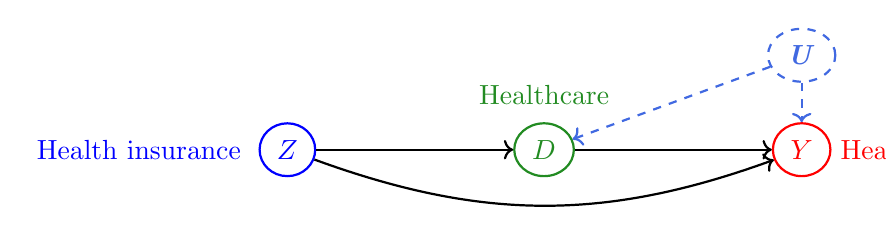
\begin{tikzpicture}
            \node[state, thick,ForestGreen] (mediator) at (0,0) {$D$};
            \node[state, thick,blue] (treatment) [left=2.5cm of mediator] {$Z$};
            \node[state, thick,red] (outcome) [right=2.5cm of mediator] {$Y$};
            % Label Z, D, Y
            \node[color=ForestGreen] [above=0.1cm of mediator] {Healthcare};
            \node[color=blue] [left=0.1cm of treatment] {Health insurance};
            \node[text width=0.1cm, color=red] [right=-0.01cm of outcome] {Health};
            % Draw the causal arrows
            \path[->, thick] (treatment) edge (mediator);
            \path[->, thick] (mediator) edge (outcome);
            \path[->, thick] (treatment) edge[bend right=20] (outcome);
            % Label direct and indirect effect
            %\node[color=orange] [below left=-0.2cm and 0.2cm of mediator] {First-stage};
            %\node[color=orange] [below right=-0.2cm and 0.5cm of mediator] {LAIE};
            %\node[color=orange] [below=0.675cm of mediator] {Direct Effect};
            % Add in the confounders
            %\node[state, thick,RoyalPurple] (confounderX) [above=1.5cm of mediator] {$\vec{X}$};
            %\path[->,RoyalPurple] (confounderX) edge (mediator);
            %\node[color=RoyalPurple] [left=0.1cm of confounderX] {Observed controls};
            \node[state, thick,dashed,thick,RoyalBlue] (confounderU) [
                above=0.5cm of outcome] {$\vec U$};
            \path[->,thick,dashed,color=RoyalBlue] (confounderU) edge (mediator);
            \path[->,thick,dashed,color=RoyalBlue] (confounderU) edge (outcome);
            %\node[color=RoyalBlue] [right=0.1cm of confounderU] {Unobserved confounder};
        \end{tikzpicture}
    \end{figure}
\end{frame}
%-------------------------------------------------------------------------------
\begin{frame}[noframenumbering]
    \frametitle{Direct \& Indirect Effects --- Selection}
    In practice, the only way to believe the \textbf{SI} assumption (selection-on-observables) is to study a case with another natural experiment for $D_i$ --- in addition to the one that guaranteed $Z_i$ is ignorable.
    \vskip-0.5cm
    \begin{figure}[h!]
        \centering
        \singlespacing
        \begin{subfigure}[c]{0.475\textwidth}
            \centering
            \caption{Cells in a lab
                $\to$ \textbf{SI} believable.}
            %%
\includegraphics[width=\textwidth]{presentation-files/headlines/science-lab.png}
        \end{subfigure}
        \begin{subfigure}[c]{0.475\textwidth}
            \centering
            \caption{People choosing healthcare
                $\to$ \textbf{SI} not.}
            %%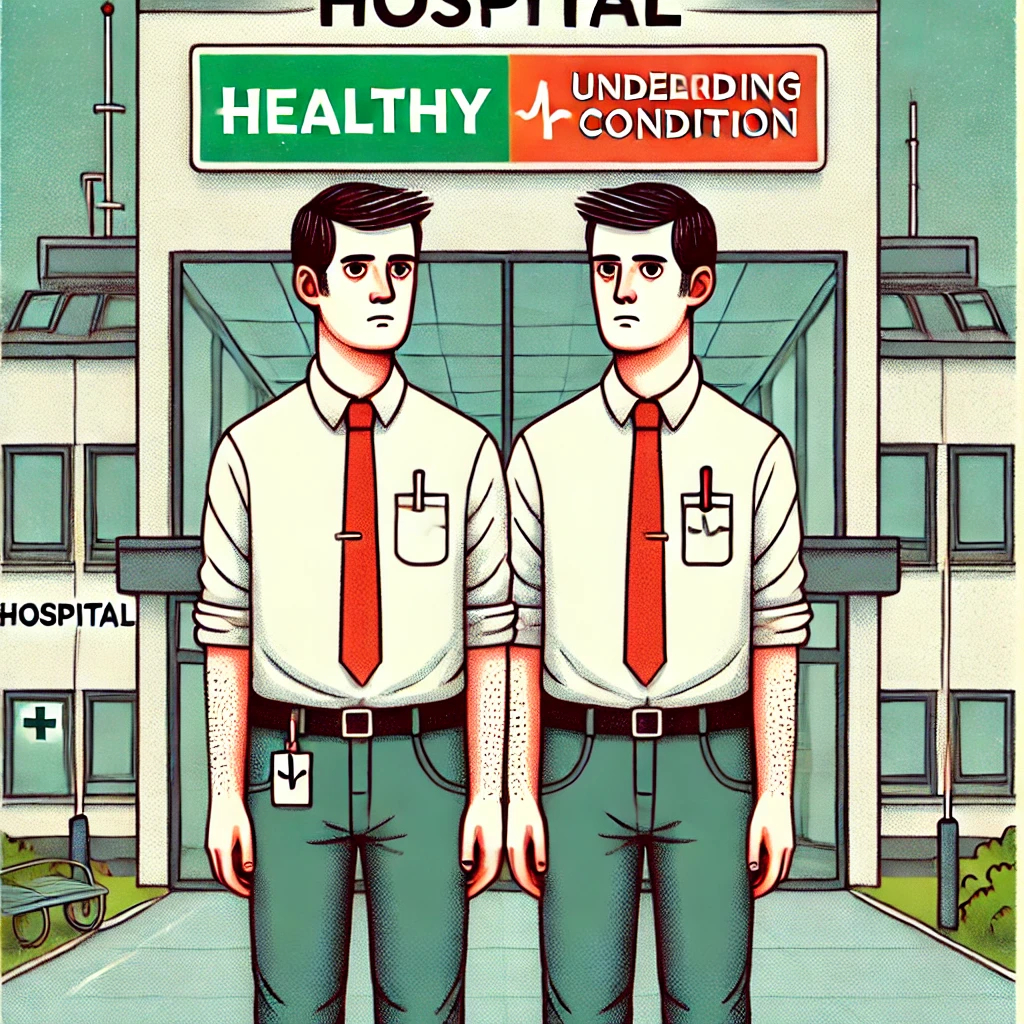
\includegraphics[width=0.965\textwidth]{presentation-files/headlines/health-differences.jpg}
        \end{subfigure}
    \end{figure}
\end{frame}
%-------------------------------------------------------------------------------
\begin{frame}
    \frametitle{Direct \& Indirect Effects --- Selection Bias}
    \begin{itemize}
        \item What happens if you go ahead and estimate CM anyway?
        \item Would this be problematic?
        \item Estimating causal effects with an unobserved confounder is usually bad$\hdots$.
    \end{itemize}
    \par\noindent\rule{\textwidth}{0.4pt}
    \vskip0.25cm
    \textbf{Definition:} Selection bias (Heckman Ichimura Smith Todd, 1998).
    \vskip0.25cm
    Estimating $D \to Y$, if $D$ not ignorable:
    \begin{align*}
        &\Egiven{ Y_i}{D_i =1} - \Egiven{ Y_i}{D_i =0} \\
        &= \text{ATT} \\
        &\;\;\;\; + \underbrace{\Big(
            \Egiven{ Y_i(.,0)}{D_i =1} - \Egiven{ Y_i(.,0)}{D_i =0} \Big)}_{
                \text{Selection Bias}}.
    \end{align*}
    \vskip1.125cm
\end{frame}
%-------------------------------------------------------------------------------
\begin{frame}[noframenumbering]
    \frametitle{Direct \& Indirect Effects --- Selection Bias}
    \begin{itemize}
        \item What happens if you go ahead and estimate CM anyway?
        \item Would this be problematic?
        \item Estimating causal effects with an unobserved confounder is usually bad$\hdots$.
    \end{itemize}
    \par\noindent\rule{\textwidth}{0.4pt}
    \vskip0.25cm
    \textbf{Definition:} Selection bias (Heckman Ichimura Smith Todd, 1998).
    \vskip0.25cm
    Estimating $D \to Y$, if $D$ not ignorable:
    \begin{align*}
        &\Egiven{ Y_i}{D_i =1} - \Egiven{ Y_i}{D_i =0} \\
        &= \text{ATE} \\
        &\;\;\;\; + \underbrace{\Big(
            \Egiven{ Y_i(., 0)}{D_i =1} - \Egiven{ Y_i(.,0)}{D_i =0} \Big)}_{
                \text{Selection Bias}} \\
        &\;\;\;\;+ \underbrace{ \Prob{D_i=0} (\text{ATT}- \text{ATU}) }_{
            \text{Group-differences Bias}}.
    \end{align*}
\end{frame}
%-------------------------------------------------------------------------------
\begin{frame}[noframenumbering]
    \frametitle{Direct \& Indirect Effects --- Selection Bias}
    \label{main:ade-selection-bias}
    $\implies$ CM Effects have this same flavour, causal effects contaminated by (less interpretable) bias terms.
    \hyperlink{cm-model}{\beamergotobutton{Model}}
    \[ \text{\textcolor{purple}{CM Estimand}}
        = \text{\textcolor{blue}{ADE}}
            + \Big(\text{\textcolor{red}{Selection Bias}}
            + \text{\textcolor{orange}{Group difference bias}}\Big) \]
    \vspace{-0.25cm}
    {\footnotesize
    \begin{align*}
        & \underbrace{\mathbb E_{D_i=d'} \Big[
            \Egiven{Y_i}{Z_i = 1, D_i=d'} - \Egiven{Y_i}{Z_i = 0, D_i=d'} \Big]}_{
                \text{\textcolor{purple}{Estimand, Direct Effect}} } \\
        & = \underbrace{\E{Y_i(1, D_i(Z_i)) - Y_i(0, D_i(Z_i))}}_{
            \text{\textcolor{blue}{Average Direct Effect}}} \\
        & \;\;\;\; + \underbrace{ \mathbb E_{D_i=d'} \Big[ 
            \Egiven{Y_i(0, D_i(Z_i))}{D_i(1) = d'} 
            - \Egiven{Y_i(0, D_i(Z_i))}{D_i(0) = d'} \Big] }_{
                \text{\textcolor{red}{Selection Bias}}} \\
        & \;\;\;\; + \underbrace{ \E[D_i =d']{
            \begin{aligned}
            &\Big(1 - \Prob{D_i(1) = d'} \Big) \\
            &\times \left( \begin{aligned}
                &\Egiven{Y_i(1, D_i(Z_i)) - Y_i(0, D_i(Z_i))}{D_i(1) = 1-d'} \\ 
                &  - \Egiven{Y_i(1, D_i(Z_i)) - Y_i(0, D_i(Z_i))}{D_i(0) = d'}
                \end{aligned} \right) \end{aligned}} }_{
                    \text{\textcolor{orange}{Group difference bias}}}
    \end{align*}}
    \hyperlink{group-diff-ade}{\beamergotobutton{Group-diff}}
\end{frame}
%-------------------------------------------------------------------------------
\begin{frame}[noframenumbering]
    \frametitle{Direct \& Indirect Effects --- Selection Bias}
    \label{main:aie-selection-bias}
    $\implies$ CM Effects have this same flavour, causal effects contaminated by (less interpretable) bias terms.
    \hyperlink{cm-model}{\beamergotobutton{Model}}
    Put $\pi = \Prob{D_i(1) = 1, D_i(0) = 0}$.
    \[ \text{\textcolor{purple}{CM Estimand}}
        = \text{\textcolor{ForestGreen}{AIE}}
            + \Big(\text{\textcolor{red}{Selection Bias}}
            + \text{\textcolor{orange}{Group difference bias}}\Big) \]
    \vspace{-0.25cm}
    {\footnotesize
    \begin{align*}
        & \underbrace{\E[Z_i]{
            \Big( \Egiven{D_i}{Z_i = 1} - \Egiven{D_i}{Z_i = 0} \Big) \times
            \Big( \Egiven{Y_i}{Z_i, D_i = 1} - \Egiven{Y_i}{Z_i, D_i = 0} \Big) }}_{ \text{\textcolor{purple}{Estimand, Indirect Effect}} } \\
        & = \underbrace{\E{Y_i(Z_i, D_i(1)) - Y_i(Z_i, D_i(0))}}_{
            \text{\textcolor{ForestGreen}{Average Indirect Effect}} } \\
        & \;\;\;\; + \underbrace{\pi  \Big(
            \Egiven{Y_i(Z_i, 0)}{D_i = 1} - \Egiven{Y_i(Z_i, 0)}{D_i = 0} \Big)}_{
                \text{\textcolor{red}{Selection Bias}}} \\
        %& \;\;\;\; + \Prob{D_i(1) = 1, D_i(0) = 0} \times \\
        %& \;\;\;\; \;\; \underbrace{ \left[ \begin{aligned}
        & \;\;\;\; + \underbrace{ \pi \left[ \begin{aligned}
            &\Big( 1 - \Prob{D_i=1} \Big)
            \left( \begin{aligned}
                &\Egiven{Y_i(Z_i, 1) - Y_i(Z_i, 0)}{D_i = 1} \\ 
                &  - \Egiven{Y_i(Z_i, 1) - Y_i(Z_i, 0)}{D_i = 0}
            \end{aligned} \right) \\
            &+ \left( \frac{1 - \Prob{D_i(1) = 1, D_i(0) = 0} }{
                \Prob{D_i(1) = 1, D_i(0) = 0}} \right)
            \left( \begin{aligned}
                &\Egiven{Y_i(Z_i, 1) - Y_i(Z_i, 0)}{D_i(1) = 0 \text{ or } D_i(0)=1} \\ 
                &  - \E{Y_i(Z_i, 1) - Y_i(Z_i, 0)}
            \end{aligned} \right)
        \end{aligned} \right]}_{\text{\textcolor{orange}{
            Groups difference Bias
                \hyperlink{group-diff-aie}{\beamergotobutton{Group-diff}}}}}
    \end{align*}}
\end{frame}
%-------------------------------------------------------------------------------
\section{3. Control Function}
%-------------------------------------------------------------------------------
\begin{frame}
    \frametitle{Identification Under Selection}
    That was a long way of giving negative results.
    Is there any hope?
    \par\noindent\rule{\textwidth}{0.4pt}
    \vskip0.25cm
    If you can use a two-way research design, then please do!
    \begin{figure}
        \centering
        \singlespacing
        \caption{Two-way Diff-in-Diff (see Deuchert Huber Schelker, 2019).}
        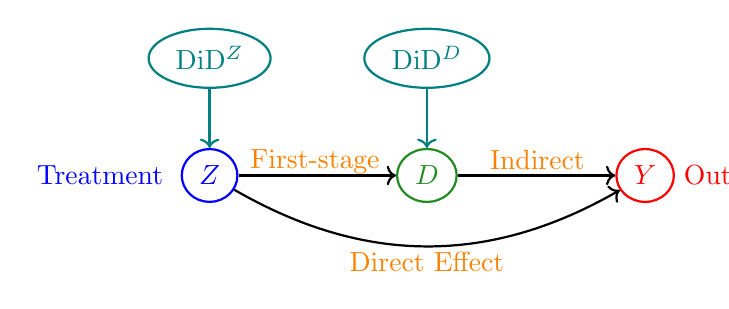
\begin{tikzpicture}
            \node[state, thick,ForestGreen] (mediator) at (0,0) {$D$};
            \node[state, thick,blue] (treatment) [left=2cm of mediator] {$Z$};
            \node[state, thick,red] (outcome) [right=2cm of mediator] {$Y$};
            % Label Z, D, Y
            %\node[color=ForestGreen] [above=0.1cm of mediator] {Mediator};
            \node[color=blue] [left=0.1cm of treatment] {Treatment};
            \node[text width=0.1cm, color=red] [right=-0.01cm of outcome] {Outcome};
            % Draw the causal arrows
            \path[->, thick] (treatment) edge (mediator);
            \path[->, thick] (mediator) edge (outcome);
            \path[->, thick] (treatment) edge[bend right=30] (outcome);
            % Label direct and indirect effect
            \node[color=orange] [above left=-0.35cm and 0.2cm of mediator] {First-stage};
            \node[color=orange] [above right=-0.3cm and 0.4cm of mediator] {Indirect};
            \node[color=orange] [below=0.5cm of mediator] {Direct Effect};
            % Add in the DiD strategy.
            \node[state, thick,teal] (DiD-Z) [above=0.75cm of treatment] {DiD$^Z$};
            \node[state, thick,teal] (DiD-D) [above=0.75cm of mediator] {DiD$^D$};
            \path[->, thick, teal] (DiD-Z) edge (treatment);
            \path[->, thick, teal] (DiD-D) edge (mediator);
            %\node[state, thick,RoyalPurple] (confounderX) [above=1.5cm of mediator] {$\vec{X}$};
            %\path[->,RoyalPurple] (confounderX) edge (mediator);
            %\node[color=RoyalPurple] [left=0.1cm of confounderX] {Observed controls};
            %\node[state, thick,dashed,RoyalBlue] (confounderU) [above=0.75cm of outcome] {$\vec U$};
            %\path[->,dashed,color=RoyalBlue] (confounderU) edge (mediator);
            %\path[->,dashed,color=RoyalBlue] (confounderU) edge (outcome);
            %\node[color=RoyalBlue] [right=0.1cm of confounderU] {Unobserved confounder};
        \end{tikzpicture}
    \end{figure}
    \textbf{Note:} assumes common trends across complier groups, identifies ADE $+$ AIE local to complier groups.
\end{frame}
%-------------------------------------------------------------------------------
\begin{frame}[noframenumbering]
    \frametitle{Identification Under Selection}
    That was a long way of giving negative results.
    Is there any hope?
    \par\noindent\rule{\textwidth}{0.4pt}
    \vskip0.25cm
    If you can use a two-way research design, then please do!
    \begin{figure}
        \centering
        \singlespacing
        \caption{Two-way IV (see Frl\"olich Huber, 2017).}
        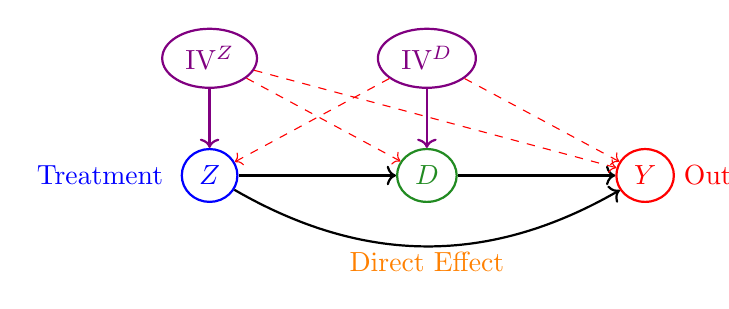
\begin{tikzpicture}
            \node[state, thick,ForestGreen] (mediator) at (0,0) {$D$};
            \node[state, thick,blue] (treatment) [left=2cm of mediator] {$Z$};
            \node[state, thick,red] (outcome) [right=2cm of mediator] {$Y$};
            % Label Z, D, Y
            %\node[color=ForestGreen] [above=0.1cm of mediator] {Mediator};
            \node[color=blue] [left=0.1cm of treatment] {Treatment};
            \node[text width=0.1cm, color=red] [right=-0.01cm of outcome] {Outcome};
            % Draw the causal arrows
            \path[->, thick] (treatment) edge (mediator);
            \path[->, thick] (mediator) edge (outcome);
            \path[->, thick] (treatment) edge[bend right=30] (outcome);
            % Label direct and indirect effect
            \node[color=orange] [below=0.5cm of mediator] {Direct Effect};
            % Add in the IV strategy.
            \node[state, thick,violet] (IV-Z) [above=0.75cm of treatment] {IV$^Z$};
            \node[state, thick,violet] (IV-D) [above=0.75cm of mediator] {IV$^D$};
            \path[->, thick,   violet] (IV-Z) edge (treatment);
            \path[->, thick,   violet] (IV-D) edge (mediator);
            % and the exclusion restrictions
            
            \path[->, dashed, red] (IV-Z) edge (mediator);
            \path[->, dashed, red] (IV-Z) edge (outcome);
            
            \path[->, dashed, red] (IV-D) edge (treatment);
            \path[->, dashed, red] (IV-D) edge (outcome);
            %\node[state, thick,RoyalPurple] (confounderX) [above=1.5cm of mediator] {$\vec{X}$};
            %\path[->,RoyalPurple] (confounderX) edge (mediator);
            %\node[color=RoyalPurple] [left=0.1cm of confounderX] {Observed controls};
            %\node[state, thick,dashed,RoyalBlue] (confounderU) [above=0.75cm of outcome] {$\vec U$};
            %\path[->,dashed,color=RoyalBlue] (confounderU) edge (mediator);
            %\path[->,dashed,color=RoyalBlue] (confounderU) edge (outcome);
            %\node[color=RoyalBlue] [right=0.1cm of confounderU] {Unobserved confounder};
        \end{tikzpicture}
    \end{figure}
    \textbf{Note:} two-way exclusion restriction, identifies ADE $+$ AIE local to overlapping complier groups.
    Also avoid 2SLS (see Kim 2025)!
\end{frame}
%-------------------------------------------------------------------------------
\begin{frame}[noframenumbering]
    \frametitle{Identification Under Selection}
    That was a long way of giving negative results.
    Is there any hope?
    \par\noindent\rule{\textwidth}{0.4pt}
    \vskip0.25cm
    What about the mainstream case, with research design for only $Z$?\\
    How do economists do causal effects in these systems?
    \begin{enumerate}
        \item Estimate the ATE, and call it a day.
        \item (optional) Present suggestive evidence of mechanisms$\hdots$.
        \hyperlink{suggestive-evidence}{\beamergotobutton{Suggestive}}
    \end{enumerate}
    \vskip0.5cm
    \par\noindent\rule{\textwidth}{0.4pt}
    \vfill
    \textbf{New:} Control Function solution to identification.
\end{frame}
%-------------------------------------------------------------------------------
\begin{frame}
    \frametitle{Identification with a Control Function}
    Suppose $Z$ is ignorable, $D$ is not, so we have the following causal model.
    \vskip-0.75cm
    \begin{figure}
        \centering
        \singlespacing
        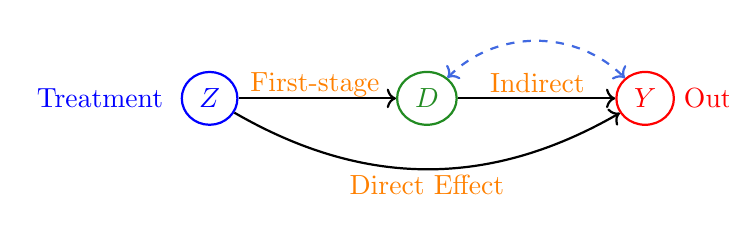
\begin{tikzpicture}
            \node[state, thick,ForestGreen] (mediator) at (0,0) {$D$};
            \node[state, thick,blue] (treatment) [left=2cm of mediator] {$Z$};
            \node[state, thick,red] (outcome) [right=2cm of mediator] {$Y$};
            % Label Z, D, Y
            %\node[color=ForestGreen] [above=0.1cm of mediator] {Mediator};
            \node[color=blue] [left=0.1cm of treatment] {Treatment};
            \node[text width=0.1cm, color=red] [right=-0.01cm of outcome] {Outcome};
            % Draw the causal arrows
            \path[->, thick] (treatment) edge (mediator);
            \path[->, thick] (mediator) edge (outcome);
            \path[->, thick] (treatment) edge[bend right=30] (outcome);
            % Label direct and indirect effect
            \node[color=orange] [above left=-0.35cm and 0.2cm of mediator] {First-stage};
            \node[color=orange] [above right=-0.3cm and 0.4cm of mediator] {Indirect};
            \node[color=orange] [below=0.5cm of mediator] {Direct Effect};
            % Add in the unobserved confounding
            \path[<->,dashed,thick,color=RoyalBlue] (mediator) edge[bend right=-45] (outcome);
        \end{tikzpicture}
    \end{figure}
    \vskip-0.25cm
    Write outcomes as sum of means and mean-zero errors, $U_{D_i , i}$.
    \[ Y_i(Z_i, 0)
        = \Egiven{Y_i(Z_i, 0)}{\vec X_i} + U_{0,i}, \;\;
    Y_i(Z_i, 1)
        = \Egiven{Y_i(Z_i, 1)}{\vec X_i} + U_{1,i}. \]
    \par\noindent\rule{\textwidth}{0.4pt}
    Then this system has the following regression equations:
    \begin{align*}
        D_i &= \phi + \pi Z_i + \varphi(\vec X_i) + U_i  \\
        Y_i &= \alpha + \beta D_i + \gamma Z_i + \delta Z_i D_i
        + \zeta(\vec X_i)
        + \underbrace{\left(1 - D_i \right)U_{0,i} + D_i U_{1,i}}_{
            \text{Correlated error term.}}
    \end{align*}
    \vskip-0.5cm
    Where $\beta, \gamma, \delta, \pi$ comprise the ADE and AIE.
\end{frame}
%-------------------------------------------------------------------------------
\begin{frame}[noframenumbering]
    \frametitle{Identification with a Control Function}
    Suppose $Z$ is ignorable, $D$ is not, so we have the following causal model.
    \vskip-0.75cm
    \begin{figure}
        \centering
        \singlespacing
        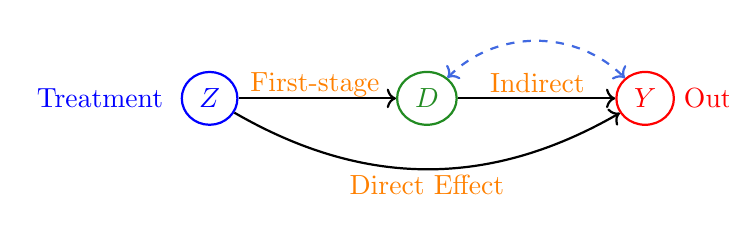
\begin{tikzpicture}
            \node[state, thick,ForestGreen] (mediator) at (0,0) {$D$};
            \node[state, thick,blue] (treatment) [left=2cm of mediator] {$Z$};
            \node[state, thick,red] (outcome) [right=2cm of mediator] {$Y$};
            % Label Z, D, Y
            %\node[color=ForestGreen] [above=0.1cm of mediator] {Mediator};
            \node[color=blue] [left=0.1cm of treatment] {Treatment};
            \node[text width=0.1cm, color=red] [right=-0.01cm of outcome] {Outcome};
            % Draw the causal arrows
            \path[->, thick] (treatment) edge (mediator);
            \path[->, thick] (mediator) edge (outcome);
            \path[->, thick] (treatment) edge[bend right=30] (outcome);
            % Label direct and indirect effect
            \node[color=orange] [above left=-0.35cm and 0.2cm of mediator] {First-stage};
            \node[color=orange] [above right=-0.3cm and 0.4cm of mediator] {Indirect};
            \node[color=orange] [below=0.5cm of mediator] {Direct Effect};
            % Add in the unobserved confounding
            \path[<->,dashed,thick,color=RoyalBlue] (mediator) edge[bend right=-45] (outcome);
        \end{tikzpicture}
    \end{figure}
    \vskip-0.25cm

    \par\noindent\rule{\textwidth}{0.4pt}
    Then this system has the following regression equations:
    \begin{align*}
        D_i &= \phi + \pi Z_i + \varphi(\vec X_i) + U_i  \\
        Y_i &= \alpha + \beta D_i + \gamma Z_i + \delta Z_i D_i
        + \zeta(\vec X_i)
        + \underbrace{\left(1 - D_i \right)U_{0,i} + D_i U_{1,i}}_{
            \text{Correlated error term.}}
    \end{align*}
    \vskip-0.5cm
    Where $\beta, \gamma, \delta, \pi$ comprise the ADE and AIE.
    \vfill
    
    \par\noindent\rule{\textwidth}{0.4pt}
    \textbf{Control Function intuition:} Identify second-stage (despite correlated error term), to get ADE $+$ AIE.
\end{frame}
%-------------------------------------------------------------------------------
\begin{frame}[noframenumbering]
    \frametitle{Identification with a Control Function}
    Suppose $Z$ is ignorable, $D$ is not, so we have the following causal model.
    \vskip-0.75cm
    \begin{figure}
        \centering
        \singlespacing
        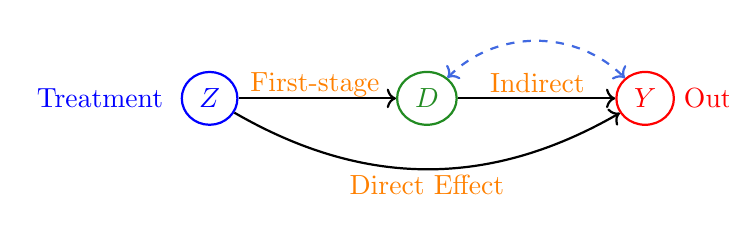
\begin{tikzpicture}
            \node[state, thick,ForestGreen] (mediator) at (0,0) {$D$};
            \node[state, thick,blue] (treatment) [left=2cm of mediator] {$Z$};
            \node[state, thick,red] (outcome) [right=2cm of mediator] {$Y$};
            % Label Z, D, Y
            %\node[color=ForestGreen] [above=0.1cm of mediator] {Mediator};
            \node[color=blue] [left=0.1cm of treatment] {Treatment};
            \node[text width=0.1cm, color=red] [right=-0.01cm of outcome] {Outcome};
            % Draw the causal arrows
            \path[->, thick] (treatment) edge (mediator);
            \path[->, thick] (mediator) edge (outcome);
            \path[->, thick] (treatment) edge[bend right=30] (outcome);
            % Label direct and indirect effect
            \node[color=orange] [above left=-0.35cm and 0.2cm of mediator] {First-stage};
            \node[color=orange] [above right=-0.3cm and 0.4cm of mediator] {Indirect};
            \node[color=orange] [below=0.5cm of mediator] {Direct Effect};
            % Add in the unobserved confounding
            \path[<->,dashed,thick,color=RoyalBlue] (mediator) edge[bend right=-45] (outcome);
        \end{tikzpicture}
    \end{figure}
    \vskip-0.25cm

    \par\noindent\rule{\textwidth}{0.4pt}
    \textbf{Note:} Roy selection has first- and second-stage errors correlated.
    \begin{align*}
        D_i &= \indicator{
            Z_i(\delta + \beta) + (1 - Z_i)\beta
                \geq C_i - 
                \Big(\eqhighlight{yellow}{U_{1,i} - U_{0,i}} \Big) } \\
        Y_i &= \alpha + \beta D_i + \gamma Z_i + \delta Z_i D_i
        + \zeta(\vec X_i)
        + \underbrace{\eqhighlight{yellow}{
            \left(1 - D_i \right)U_{0,i} + D_i U_{1,i}}}_{
            \text{Correlated error term}}
    \end{align*}
    where $C_i$ are costs of taking $D_i$.
    \par\noindent\rule{\textwidth}{0.4pt}
    \textbf{Control Function intuition:} use first-stage errors to purge second-stage correlated errors.
\end{frame}
%-------------------------------------------------------------------------------
\begin{frame}
    \frametitle{Identification with a Control Function}
    Suppose $Z$ is ignorable, $D$ is not, so we have the following causal model.
    \vskip-0.75cm
    \begin{figure}
        \centering
        \singlespacing
        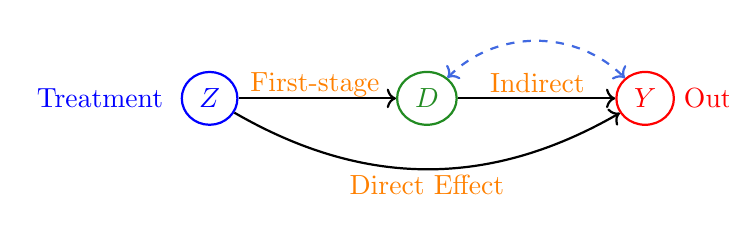
\begin{tikzpicture}
            \node[state, thick,ForestGreen] (mediator) at (0,0) {$D$};
            \node[state, thick,blue] (treatment) [left=2cm of mediator] {$Z$};
            \node[state, thick,red] (outcome) [right=2cm of mediator] {$Y$};
            % Label Z, D, Y
            %\node[color=ForestGreen] [above=0.1cm of mediator] {Mediator};
            \node[color=blue] [left=0.1cm of treatment] {Treatment};
            \node[text width=0.1cm, color=red] [right=-0.01cm of outcome] {Outcome};
            % Draw the causal arrows
            \path[->, thick] (treatment) edge (mediator);
            \path[->, thick] (mediator) edge (outcome);
            \path[->, thick] (treatment) edge[bend right=30] (outcome);
            % Label direct and indirect effect
            \node[color=orange] [above left=-0.35cm and 0.2cm of mediator] {First-stage};
            \node[color=orange] [above right=-0.3cm and 0.4cm of mediator] {Indirect};
            \node[color=orange] [below=0.5cm of mediator] {Direct Effect};
            % Add in the unobserved confounding
            \path[<->,dashed,thick,color=RoyalBlue] (mediator) edge[bend right=-45] (outcome);
        \end{tikzpicture}
    \end{figure}
    \vskip-0.25cm

    \par\noindent\rule{\textwidth}{0.4pt}
    \textbf{Heckman (1979) Control Function}, assumptions:
    \begin{itemize}
        \item Mediator monotonicity, $\Probgiven{ D_i(1) \geq D_i(0) }{\vec X_i} = 1$
        \[ \implies D_i(z') = \indicator{\mu(z';\vec X_i) \geq U_i}. \]
        \item First-stage errors inform second-stage errors, 
        \[ \text{Cov}\Big[ U_i, \left(1 - D_i \right)U_{0,i} + D_i U_{1,i} \Big] \neq 0. \]
        \item Error-term distribution,
        $U_i, U_{0,i}, U_{1,i} \sim \text{TriNormal}\left(\mat M, \mat\Sigma \right)$.
    \end{itemize}
    \vskip0.25cm
    $\implies$ identify second-stage, and thus ADE $+$ AIE.
\end{frame}
%-------------------------------------------------------------------------------
\begin{frame}[noframenumbering]
    \frametitle{Identification with a Control Function}
    Suppose $Z$ is ignorable, $D$ is not, so we have the following causal model.
    \vskip-0.75cm
    \begin{figure}
        \centering
        \singlespacing
        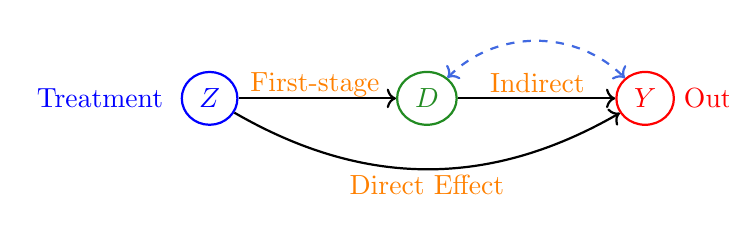
\begin{tikzpicture}
            \node[state, thick,ForestGreen] (mediator) at (0,0) {$D$};
            \node[state, thick,blue] (treatment) [left=2cm of mediator] {$Z$};
            \node[state, thick,red] (outcome) [right=2cm of mediator] {$Y$};
            % Label Z, D, Y
            %\node[color=ForestGreen] [above=0.1cm of mediator] {Mediator};
            \node[color=blue] [left=0.1cm of treatment] {Treatment};
            \node[text width=0.1cm, color=red] [right=-0.01cm of outcome] {Outcome};
            % Draw the causal arrows
            \path[->, thick] (treatment) edge (mediator);
            \path[->, thick] (mediator) edge (outcome);
            \path[->, thick] (treatment) edge[bend right=30] (outcome);
            % Label direct and indirect effect
            \node[color=orange] [above left=-0.35cm and 0.2cm of mediator] {First-stage};
            \node[color=orange] [above right=-0.3cm and 0.4cm of mediator] {Indirect};
            \node[color=orange] [below=0.5cm of mediator] {Direct Effect};
            % Add in the unobserved confounding
            \path[<->,dashed,thick,color=RoyalBlue] (mediator) edge[bend right=-45] (outcome);
        \end{tikzpicture}
    \end{figure}
    \vskip-0.25cm

    \par\noindent\rule{\textwidth}{0.4pt}
    \textbf{Heckman (1979) Control Function}, in operation:
    \begin{enumerate}
        \item Back out Control Function (CF) in first-stage (probit, normal errors),
        \[ \hat K_i = D_i -
            \hat{\mathbb E} \left[ D_i \middle\vert Z_i, \vec X_i \right].
        \]
        \item Include Mills ratio CF in OLS estimates of the second-stage,
        \[ Y_i = \alpha + \beta D_i + \gamma Z_i + \delta Z_i D_i
            + \vec \zeta' \vec X_i
            + \underbrace{\left(1 - D_i \right)\lambda\left(-\hat K_i\right)
                + D_i \lambda\left(\hat K_i\right)}_{
                \text{CF correction, $\lambda(.)$ inv Mills ratio.}}
            + \varepsilon_i \]
        \vspace{-0.5cm}
        \item Compose estimates from second-stage,
        \[ \hat{\text{ADE}}
            = \hat\gamma + \hat\delta \E{D_i}, \;\;\;\;
        \hat{\text{AIE}} 
            = \hat\pi \Big(
                \hat\beta +  \hat\delta \E{Z_i}
                + \E{\lambda\left(\hat K_i\right) -
                    \lambda\left(-\hat K_i\right)}\Big). \]
    \end{enumerate}
\end{frame}
%-------------------------------------------------------------------------------
\begin{frame}
    \frametitle{Identification with a Control Function}
    Suppose $Z$ is ignorable, $D$ is not, so we have the following causal model.
    \vskip-0.75cm
    \begin{figure}
        \centering
        \singlespacing
        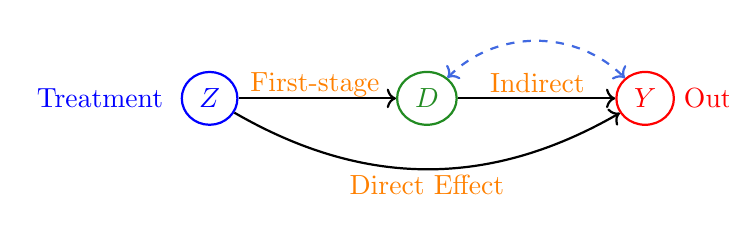
\begin{tikzpicture}
            \node[state, thick,ForestGreen] (mediator) at (0,0) {$D$};
            \node[state, thick,blue] (treatment) [left=2cm of mediator] {$Z$};
            \node[state, thick,red] (outcome) [right=2cm of mediator] {$Y$};
            % Label Z, D, Y
            %\node[color=ForestGreen] [above=0.1cm of mediator] {Mediator};
            \node[color=blue] [left=0.1cm of treatment] {Treatment};
            \node[text width=0.1cm, color=red] [right=-0.01cm of outcome] {Outcome};
            % Draw the causal arrows
            \path[->, thick] (treatment) edge (mediator);
            \path[->, thick] (mediator) edge (outcome);
            \path[->, thick] (treatment) edge[bend right=30] (outcome);
            % Label direct and indirect effect
            \node[color=orange] [above left=-0.35cm and 0.2cm of mediator] {First-stage};
            \node[color=orange] [above right=-0.3cm and 0.4cm of mediator] {Indirect};
            \node[color=orange] [below=0.5cm of mediator] {Direct Effect};
            % Add in the unobserved confounding
            \path[<->,dashed,thick,color=RoyalBlue] (mediator) edge[bend right=-45] (outcome);
        \end{tikzpicture}
    \end{figure}
    \vskip-0.25cm

    \par\noindent\rule{\textwidth}{0.4pt}
    \textbf{Semi-parametric control function} (Newey Imbens 2012), assumptions:
    \begin{enumerate}
        \item Mediator monotonicity, $\Probgiven{ D_i(1) \geq D_i(0) }{\vec X_i} = 1$
        \[ \implies D_i(z') = \indicator{\mu(z';\vec X_i) \geq U_i}. \]
        \item First-stage errors inform second-stage errors, 
        \[ \text{Cov}\Big[ U_i, \left(1 - D_i \right)U_{0,i} + D_i U_{1,i} \Big] \neq 0. \]
        \item Valid instrument $\vec X_i^\text{IV}$ for $D_i$, to separate CF functional form.
    \hyperlink{MTEs}{\beamergotobutton{MTEs}}
    \end{enumerate}
    \vskip0.25cm
    $\implies$ identifies second-stage, ADE $+$ AIE (w.out error dist assumption).
\end{frame}
%-------------------------------------------------------------------------------
\begin{frame}[noframenumbering]
    \frametitle{Identification with a Control Function}
    Suppose $Z$ is ignorable, $D$ is not, so we have the following causal model.
    \vskip-0.75cm
    \begin{figure}
        \centering
        \singlespacing
        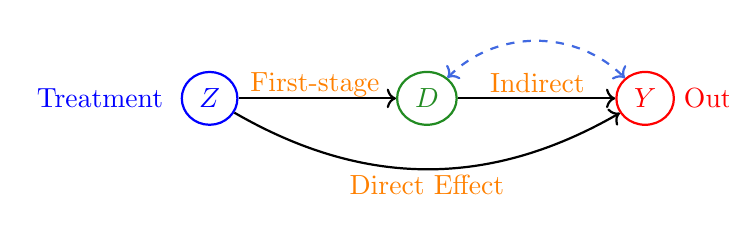
\begin{tikzpicture}
            \node[state, thick,ForestGreen] (mediator) at (0,0) {$D$};
            \node[state, thick,blue] (treatment) [left=2cm of mediator] {$Z$};
            \node[state, thick,red] (outcome) [right=2cm of mediator] {$Y$};
            % Label Z, D, Y
            %\node[color=ForestGreen] [above=0.1cm of mediator] {Mediator};
            \node[color=blue] [left=0.1cm of treatment] {Treatment};
            \node[text width=0.1cm, color=red] [right=-0.01cm of outcome] {Outcome};
            % Draw the causal arrows
            \path[->, thick] (treatment) edge (mediator);
            \path[->, thick] (mediator) edge (outcome);
            \path[->, thick] (treatment) edge[bend right=30] (outcome);
            % Label direct and indirect effect
            \node[color=orange] [above left=-0.35cm and 0.2cm of mediator] {First-stage};
            \node[color=orange] [above right=-0.3cm and 0.4cm of mediator] {Indirect};
            \node[color=orange] [below=0.5cm of mediator] {Direct Effect};
            % Add in the unobserved confounding
            \path[<->,dashed,thick,color=RoyalBlue] (mediator) edge[bend right=-45] (outcome);
        \end{tikzpicture}
    \end{figure}
    \vskip-0.5cm

    \par\noindent\rule{\textwidth}{0.4pt}
    \textbf{Semi-parametric control function} (Newey Imbens 2012), in operation:
    \begin{enumerate}
        \item Back out Control Function (CF) in first-stage (semi/non-parametric), with IV $\vec X_i^\text{IV}$,
        \vspace{-0.25cm}
        \[ \hat K_i = D_i -
            \hat{\mathbb E} \left[ D_i \middle\vert Z_i, \vec X_i^\text{IV}, \vec X_i \right].
        \]
        \item Include semi-parametric CF in OLS estimates of the second-stage,
        \[ Y_i = \alpha + \beta D_i + \gamma Z_i + \delta Z_i D_i
            + \vec \zeta' \vec X_i
            + \underbrace{\left(1 - D_i \right)\lambda_0\left(-\hat K_i\right)
                + D_i \lambda_1\left(\hat K_i\right)}_{
                \text{CF correction, $\lambda_0(.), \lambda_1(.)$ splines.}}
            + \varepsilon_i \]
        \vspace{-0.5cm}
        \item Compose estimates from second-stage,
        \[ \hat{\text{ADE}}
            = \hat\gamma + \hat\delta \E{D_i}, \;\;\;\;
        \hat{\text{AIE}}
            = \hat\pi \Big(
                \hat\beta +  \hat\delta \E{Z_i}
                + \E{\hat\lambda_0\left(\hat K_i\right) -
                    \hat\lambda_1\left(-\hat K_i\right)}\Big). \]
    \end{enumerate}
\end{frame}
%-------------------------------------------------------------------------------
\begin{frame}
    \frametitle{Simulation Evidence}
    Simulation with trivariate normal errors $+$ unobserved costs,
    $N = 10,000$.
    \vskip0cm
    \begin{enumerate}
        \item $\text{\textcolor{blue}{Random treatment $Z_i$}}
            \sim \text{Binom}\left(0.5 \right) $
        \item $ \eqhighlight{yellow}{
            \left( U_{0,i}, U_{1,i} \right) \sim
        \text{BivariateNormal}\left( 0, 0, \sigma_0, \sigma_1, \rho \right)},
            \;\; \text{Costs }C_i \sim N(0, 0.5). $
    \end{enumerate}
    \par\noindent\rule{\textwidth}{0.4pt}
    Roy \textcolor{ForestGreen}{selection-into-$D_i$}, with constant partial effects $+$ interaction term.
    \begin{align*}
        D_i(z')    &= \indicator{Y_i(z', 1) - Y_i(z', 0) \geq C_i},&  \\
        Y_i(z',d') &= \left( z' + d' + z' d' \right) + U_{d'}
        & \text{ for } z',d' = 0,1.
    \end{align*}
    \par\noindent\rule{\textwidth}{0.4pt}
    Following the previous, these data have the following first and second-stage equations, where $\vec X_i^\text{IV}$ is an additive cost IV:
    \begin{align*}
        D_i &= \indicator{Z_i - \vec X_i^{\text{IV}}
            \geq C_i - \Big(\eqhighlight{yellow}{U_{1,i} - U_{0,i}} \Big) } \\
        Y_i &= Z_i + D_i + Z_i D_i
            + \eqhighlight{yellow}{
                \left( 1 - D_i \right) U_{0,i} + D_i U_{1,i}}.
    \end{align*}
    $\implies$ unobserved confounding by BivariateNormal $\Big(U_{0,i}, U_{1,i}\Big)$.
\end{frame}
%-------------------------------------------------------------------------------
\begin{frame}[noframenumbering]
    \frametitle{Simulation Evidence}
    Simulation with Roy selection, BivariateNormal errors $+$ unobserved costs.
    \vskip-0.25cm
    \begin{figure}
        \caption{Simulated Distribution of CM Effect Estimates from 10,000 DGPs.}
        \vskip-0.25cm
        \begin{subfigure}[c]{0.475\textwidth}
            \centering
            \caption{ADE.}
            %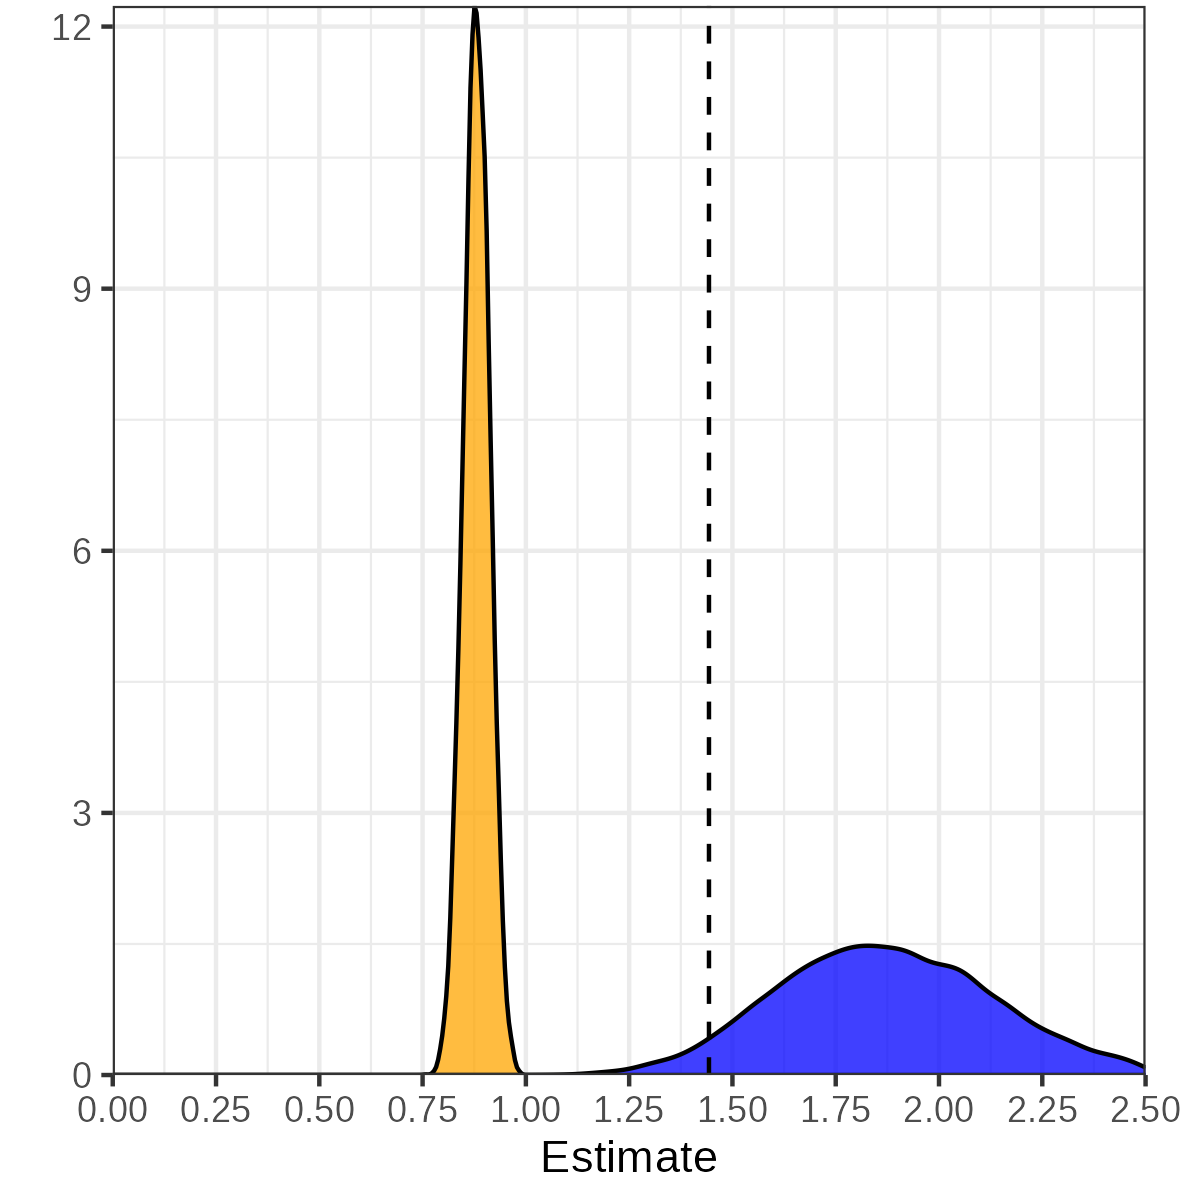
\includegraphics[width=\textwidth]{../programs/simulations/sim-output/direct-boot.png}
        \end{subfigure}
        \begin{subfigure}[c]{0.475\textwidth}
            \centering
            \caption{AIE.}
            %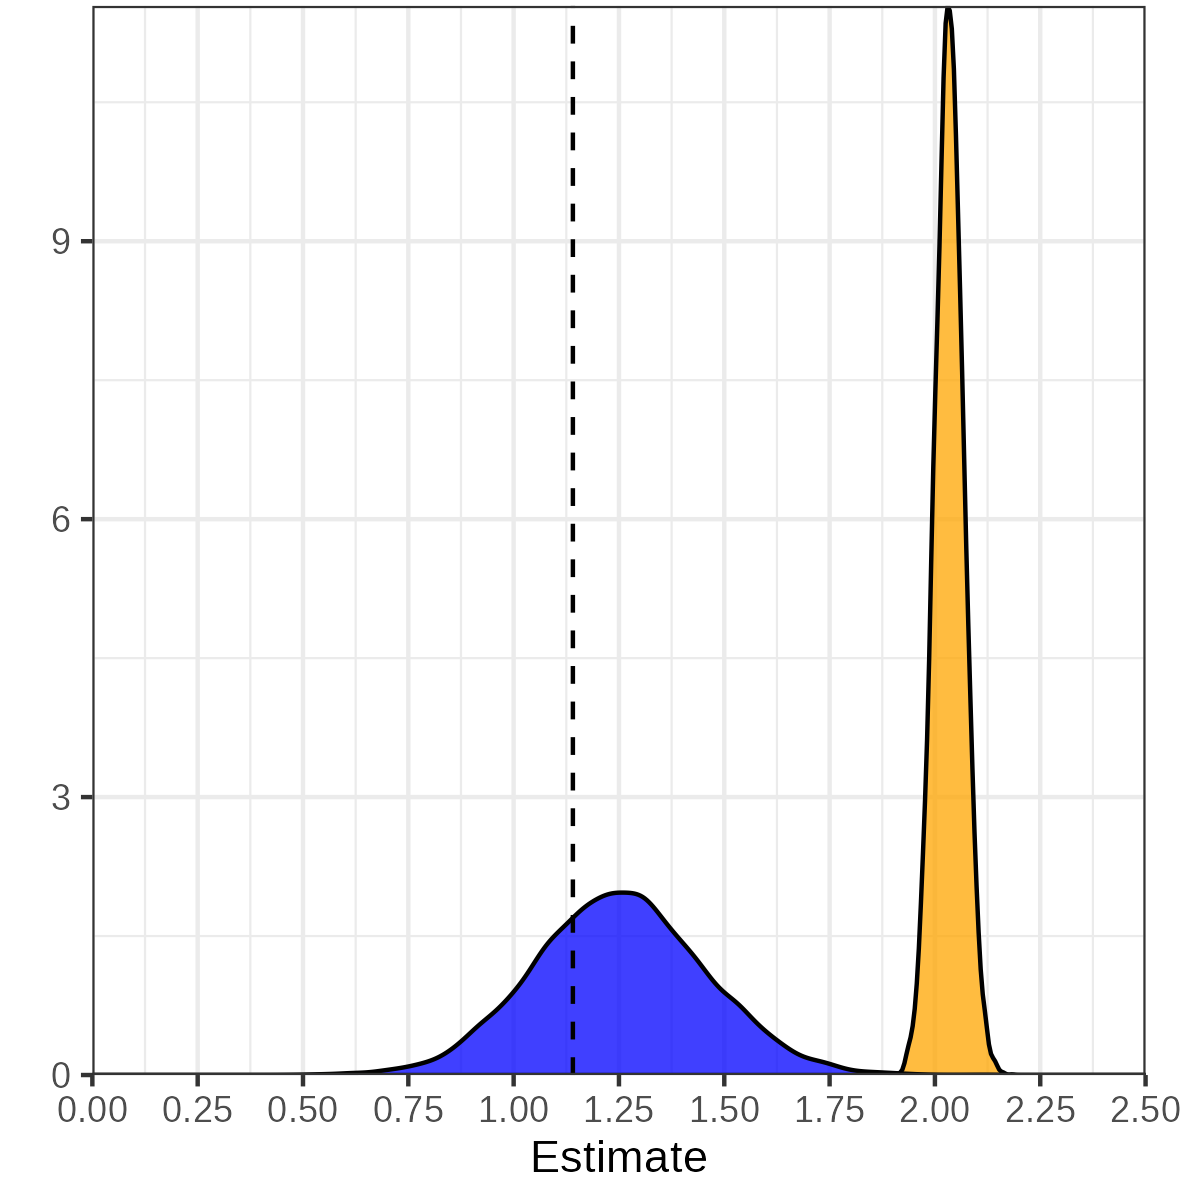
\includegraphics[width=\textwidth]{../programs/simulations/sim-output/indirect-boot.png}
        \end{subfigure}
    \end{figure}
\end{frame}
%-------------------------------------------------------------------------------
\begin{frame}[noframenumbering]
    \frametitle{Simulation Evidence}
    Simulation with Roy selection, trivariate normal errors, unobserved costs.    
    \begin{figure}[h!]
        \caption{Point Estimates of CM Effects, OLS versus Control Function, varying $\rho$ values with $\sigma_0 = 1, \sigma_1 = 2$ fixed.}
        \vskip-0.5cm
        \begin{subfigure}[c]{0.475\textwidth}
            \centering
            \caption{ADE.}
            %%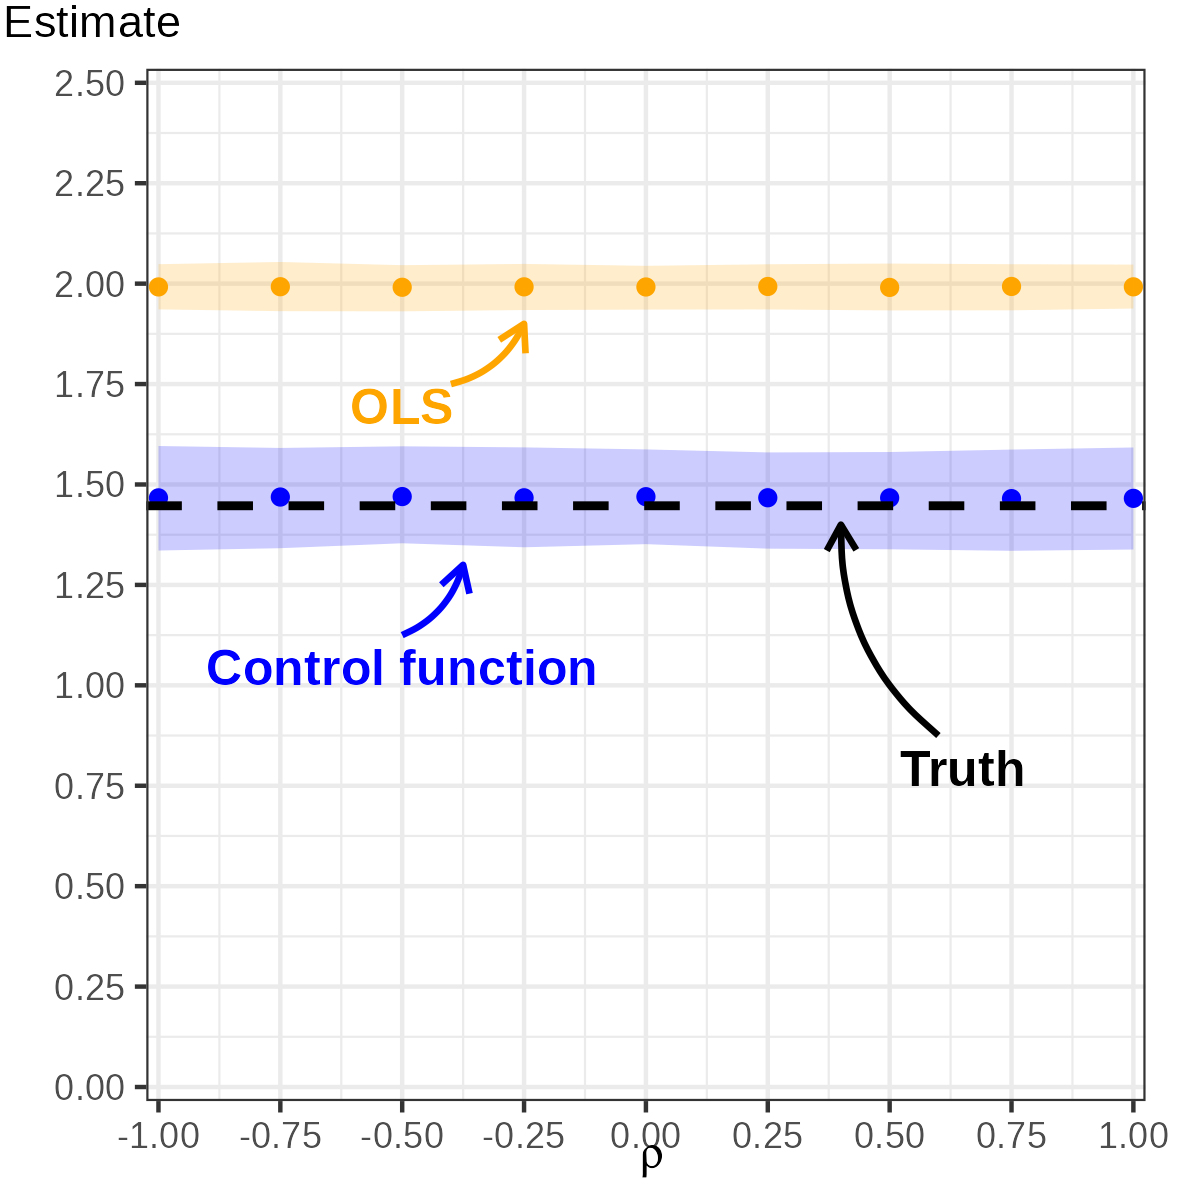
\includegraphics[width=\textwidth]{../programs/simulations/sim-output/rho-directeffect-bias.png}
        \end{subfigure}
        \begin{subfigure}[c]{0.475\textwidth}
            \centering
            \caption{AIE.}
            %%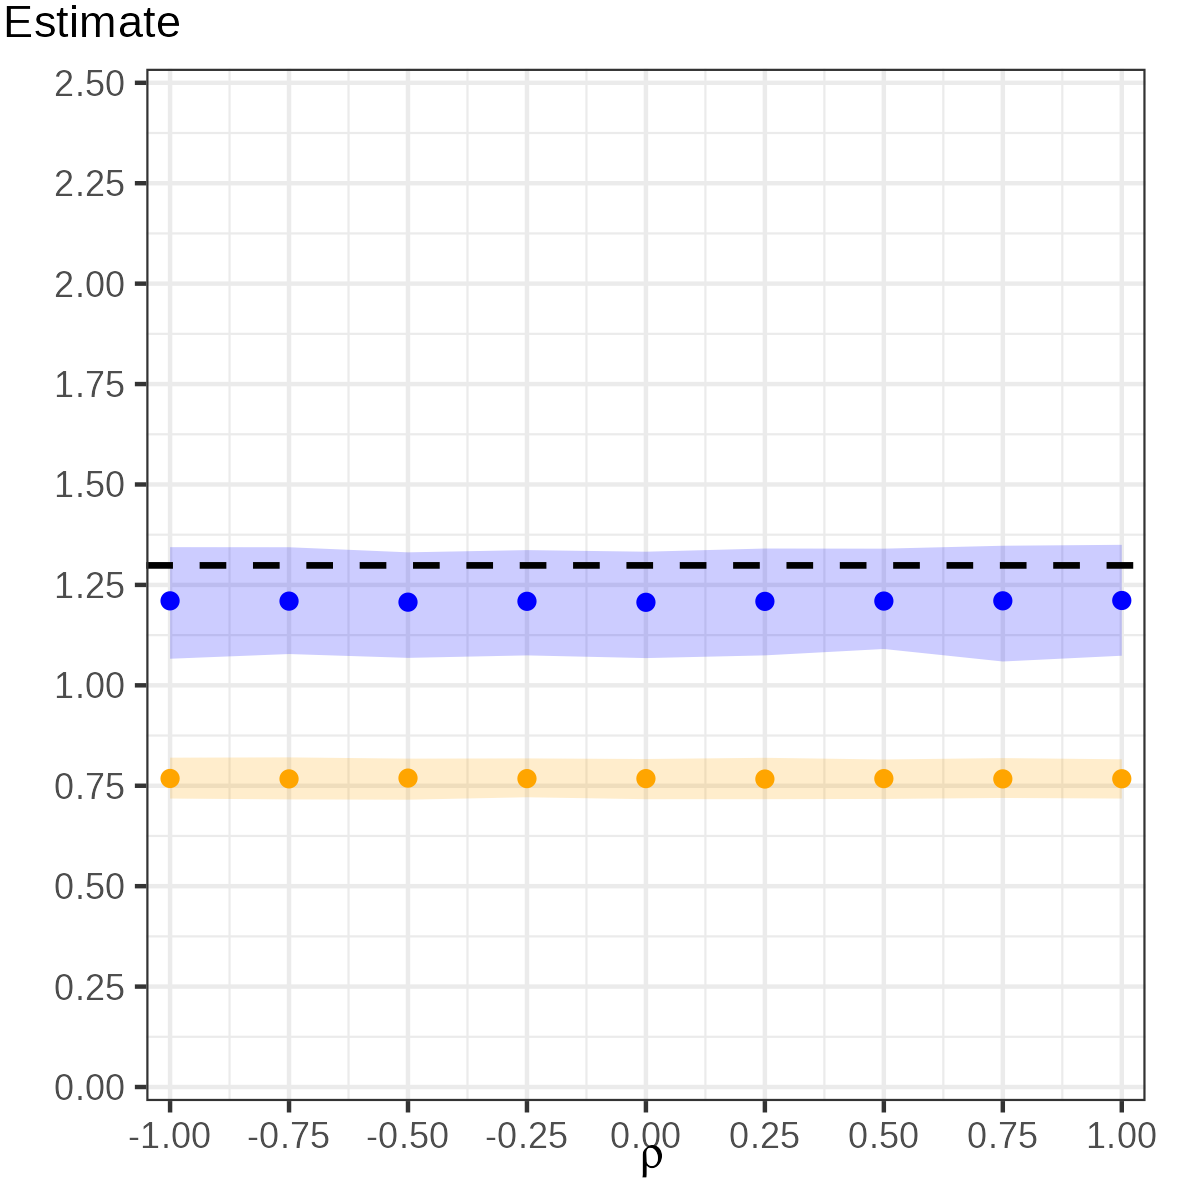
\includegraphics[width=\textwidth]{../programs/simulations/sim-output/rho-indirecteffect-bias.png}
        \end{subfigure}
    \end{figure}
\end{frame}
%-------------------------------------------------------------------------------
\section{4. Oregon}
%-------------------------------------------------------------------------------
\begin{frame}
    \frametitle{Conclusion}
    \textbf{Overarching goals:}
    \begin{enumerate}
        \item Ward economists away from using CM methods unabashedly. \\ 
        $\to$ Noted problems in the most popular methods for CM effects, pertinent for economic applications.
        \item CM methods away from ignorability assumptions, inappropriate for economics ($+$ social science) settings. \\
        $\to$ Methods valid when selection-into-treatment theory relevant.
    \end{enumerate}
    \par\noindent\rule{\textwidth}{0.4pt}
    \textbf{Work-in-progress part of LWIPS:}
    \begin{itemize}
        \item Connect the control function approach to MTE methods
        \hyperlink{MTEs}{\beamergotobutton{MTEs}}
        \item Large sample properties $+$ analytical SEs
        \item Use this approach to estimate direct and indirect effects of genetics and education (companion paper)
        \item (eventually) \textit{R} package for selection-adjusted CM effects, by Heckman model and IV-assisted CF/MTE.
    \end{itemize}
\end{frame}
%-------------------------------------------------------------------------------
\begin{frame}[noframenumbering]
    \frametitle{Appendix: CM Guiding Model}
    \label{cm-model}
    Consider binary \textcolor{blue}{treatment $Z_i = 0, 1$},
    binary \textcolor{ForestGreen}{mediator $D_i = 0, 1$},
    and continuous \textcolor{red}{outcome $Y_i$} for individuals $i = 1, \hdots, N$.
    \vskip-1.00cm
    \begin{figure}[h!]
        \centering
        \singlespacing
        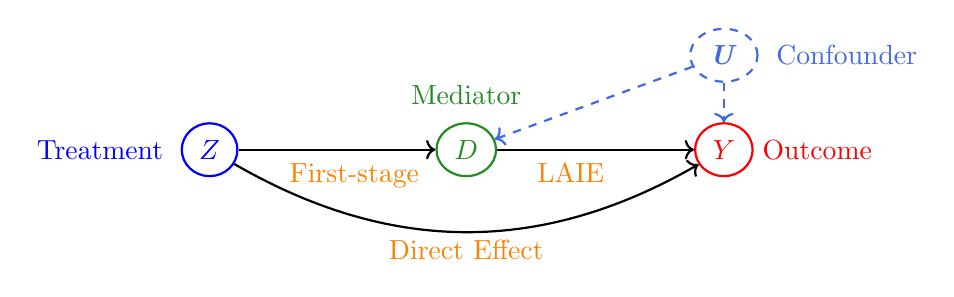
\begin{tikzpicture}
            \node[state, thick,ForestGreen] (mediator) at (0,0) {$D$};
            \node[state, thick,blue] (treatment) [left=2.5cm of mediator] {$Z$};
            \node[state, thick,red] (outcome) [right=2.5cm of mediator] {$Y$};
            % Label Z, D, Y
            \node[color=ForestGreen] [above=0.1cm of mediator] {Mediator};
            \node[color=blue] [left=0.1cm of treatment] {Treatment};
            \node[text width=0.1cm, color=red] [right=-0.01cm of outcome] {Outcome};
            % Draw the causal arrows
            \path[->, thick] (treatment) edge (mediator);
            \path[->, thick] (mediator) edge (outcome);
            \path[->, thick] (treatment) edge[bend right=30] (outcome);
            % Label direct and indirect effect
            \node[color=orange] [below left=-0.2cm and 0.2cm of mediator] {First-stage};
            \node[color=orange] [below right=-0.2cm and 0.5cm of mediator] {LAIE};
            \node[color=orange] [below=0.675cm of mediator] {Direct Effect};
            % Add in the confounders
            %\node[state, thick,RoyalPurple] (confounderX) [above=1.5cm of mediator] {$\vec{X}$};
            %\path[->,RoyalPurple] (confounderX) edge (mediator);
            %\node[color=RoyalPurple] [left=0.1cm of confounderX] {Observed controls};
            \node[state, thick,dashed,thick,RoyalBlue] (confounderU) [
                above=0.5cm of outcome] {$\vec U$};
            \node[color=RoyalBlue] [right=0.1cm of confounderU] {Confounder};
            \path[->,thick,dashed,color=RoyalBlue] (confounderU) edge (mediator);
            \path[->,thick,dashed,color=RoyalBlue] (confounderU) edge (outcome);
            %\node[color=RoyalBlue] [right=0.1cm of confounderU] {Unobserved confounder};
        \end{tikzpicture}
    \end{figure}
    \vskip-0.5cm
    \par\noindent\rule{\textwidth}{0.4pt}
    \[ \text{Average Direct Effect (ADE)}: \;\;\;
        \E{Y_i\left(\eqhighlight{blue}{1}, D_i(Z_i) \right)
            - Y_i\left(\eqhighlight{blue}{0}, D_i(Z_i) \right)} \]
    \vskip-0.35cm
    \begin{itemize}
        \item ADE is causal effect $Z\to Y$, blocking the indirect $D$ path.
    \end{itemize}
    \vskip0.25cm
    \[ \text{Average Indirect Effect (AIE):} \;\;\;
    \E{Y_i\left(Z_i, \eqhighlight{ForestGreen}{D_i(1)} \right)
        - Y_i\left(Z_i, \eqhighlight{ForestGreen}{D_i(0)} \right)} \]
    \vskip-0.25cm
    \begin{itemize}
        \item AIE is causal effect of $D(Z) \to Y$, blocking the direct $Z$ path.\footnote[frame]{
            Note: AIE $=$ fraction of $D(Z)$ compliers $\times$ average effect $D\to Y$ among compliers.}
    \end{itemize}
\end{frame}
%-------------------------------------------------------------------------------
\begin{frame}[noframenumbering]
    \frametitle{Group Difference --- ADE}
    \label{group-diff-ade}
    CM effects contaminated by (less interpretable) bias terms.
    \[ \text{\textcolor{purple}{CM Estimand}}
        = \text{\textcolor{blue}{ADEM}}
            + \text{\textcolor{red}{Selection Bias}} \]
    \vspace{-0.25cm}
    {\footnotesize
    \begin{align*}
        & \underbrace{\mathbb E_{D_i} \Big[
            \Egiven{Y_i}{Z_i = 1, D_i} - \Egiven{Y_i}{Z_i = 0, D_i} \Big]}_{
                \text{\textcolor{purple}{Estimand, Direct Effect}} } \\
        & = \underbrace{\E[D_i= d']{
            \Egiven{Y_i(1, D_i(Z_i)) - Y_i(0, D_i(Z_i))}{D_i(1) = d'}} }_{
            \text{\textcolor{blue}{Average Direct Effect on Mediator (ADEM) take-up --- i.e., $D_i(1)$ weighted}}} \\
        & \;\;\;\; + \underbrace{ \mathbb E_{D_i} \Big[ 
            \Egiven{Y_i(0, D_i(Z_i))}{D_i(1) = d'} 
            - \Egiven{Y_i(0, D_i(Z_i))}{D_i(0) = d'} \Big] }_{
                \text{\textcolor{red}{Selection Bias}}}
    \end{align*}}
    The weighted ADE you get here is a positive weighted sum of local ADEs, but with policy irrelevant weights $D_i(1) = d'$.

    \vskip0.5cm
    $\implies$ consider this group bias, noting difference from true ADE.
    \hyperlink{main:ade-selection-bias}{\beamergotobutton{Back}}
\end{frame}
%-------------------------------------------------------------------------------
\begin{frame}[noframenumbering]
    \frametitle{Group Difference --- AIE}
    \label{group-diff-aie}
    CM effects contaminated by (less interpretable) bias terms.
    \[ \text{\textcolor{purple}{CM Estimand}}
        = \text{\textcolor{ForestGreen}{AIEM}}
            + \Big(\text{\textcolor{red}{Selection Bias}}
            + \text{\textcolor{orange}{Group difference bias}}\Big) \]
    \vspace{-0.25cm}
    {\footnotesize
    \begin{align*}
        & \underbrace{\E[Z_i]{
            \Big( \Egiven{D_i}{Z_i = 1} - \Egiven{D_i}{Z_i = 0} \Big) \times
            \Big( \Egiven{Y_i}{Z_i, D_i = 1} - \Egiven{Y_i}{Z_i, D_i = 0} \Big) }}_{ \text{\textcolor{purple}{Estimand, Indirect Effect}} } \\
        & = \underbrace{
                \Egiven{Y_i(Z_i, D_i(1)) - Y_i(Z_i, D_i(0))}{D_i = 1}
            }_{\text{\textcolor{ForestGreen}{Average Indirect Effect on Mediated (AIEM) --- i.e., $D_i=1$ weighted}} } \\
        & \;\;\;\; + \underbrace{\pi  \Big(
            \Egiven{Y_i(Z_i, 0)}{D_i = 1} - \Egiven{Y_i(Z_i, 0)}{D_i = 0} \Big)}_{
                \text{\textcolor{red}{Selection Bias}}} \\
        & \;\;\;\; + \underbrace{ \pi \left[
            \left( \frac{1 - \Prob{D_i(1) = 1, D_i(0) = 0} }{
                \Prob{D_i(1) = 1, D_i(0) = 0}} \right)
            \left( \begin{aligned}
                &\Egiven{Y_i(Z_i, 1) - Y_i(Z_i, 0)}{D_i(1) = 0 \text{ or } D_i(0)=1} \\ 
                &  - \E{Y_i(Z_i, 1) - Y_i(Z_i, 0)}
            \end{aligned} \right)
        \right]}_{\text{\textcolor{orange}{Groups difference Bias}}}
    \end{align*}}
    The weighted AIE you get here is not a positive weighted sum of local AIEs, 
    because the AIE is only about $D(Z)$ compliers.
    \hyperlink{cm-model}{\beamergotobutton{Model}}.

    $\implies$ consider this group bias, noting difference from true AIE.
    \hyperlink{main:aie-selection-bias}{\beamergotobutton{Back}}
\end{frame}
%-------------------------------------------------------------------------------
\begin{frame}[noframenumbering]
    \frametitle{Appendix: Suggestive Evidence of Mechanisms}
    \label{suggestive-evidence}
    How empirical economists currently give evidence for mechanisms/mediators in causal effects.
    \vskip-0.5cm
    \begin{figure}
        \centering
        \singlespacing
        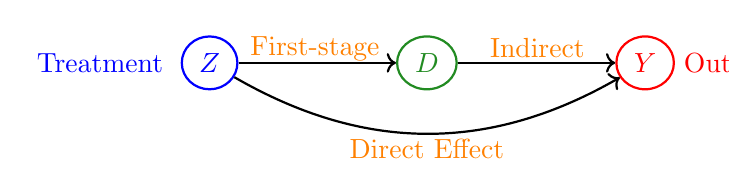
\begin{tikzpicture}
            \node[state, thick,ForestGreen] (mediator) at (0,0) {$D$};
            \node[state, thick,blue] (treatment) [left=2cm of mediator] {$Z$};
            \node[state, thick,red] (outcome) [right=2cm of mediator] {$Y$};
            % Label Z, D, Y
            %\node[color=ForestGreen] [above=0.1cm of mediator] {Mediator};
            \node[color=blue] [left=0.1cm of treatment] {Treatment};
            \node[text width=0.1cm, color=red] [right=-0.01cm of outcome] {Outcome};
            % Draw the causal arrows
            \path[->, thick] (treatment) edge (mediator);
            \path[->, thick] (mediator) edge (outcome);
            \path[->, thick] (treatment) edge[bend right=30] (outcome);
            % Label direct and indirect effect
            \node[color=orange] [above left=-0.35cm and 0.2cm of mediator] {First-stage};
            \node[color=orange] [above right=-0.3cm and 0.4cm of mediator] {Indirect};
            \node[color=orange] [below=0.5cm of mediator] {Direct Effect};
        \end{tikzpicture}
    \end{figure}
    \vskip-0.75cm
    Two causal effects are identified:
    \begin{align*}
    \text{ATE:} \;\; \E{Y_i(1, D_i(1)) - Y_i(0, D_i(0))}
        &= \Egiven{Y_i}{Z_i = 1} - \Egiven{Y_i}{Z_i = 0} \\
    \text{Average first-stage:} \;\; \E{D_i(1) - D_i(0)}
        &=\Egiven{D_i}{Z_i = 1} - \Egiven{D_i}{Z_i = 0}
    \end{align*}
    $\implies$ Show results of these two effects and assume indirect effect is positive, constant $\to$ suggestive evidence of mechanisms! 
    \vskip0.25cm
    \par\noindent\rule{\textwidth}{0.4pt}
    See Blackwell Matthew Ruofan Opacic (2024) for this in full, and a partial identification approach to avoid its unrealistic assumptions.
    % Example of this approach: the abstract of Carvahlo (2024).
\end{frame}
%-------------------------------------------------------------------------------
\begin{frame}[noframenumbering]
    \frametitle{Appendix: Connection to MTEs}
    \label{MTEs}
    The ADE is fine to estimate with a Control Function/CF, but AIE refers to mediator benefits only among mediator compliers.
    \[ \text{AIE } =
    \E{D_i(1) \neq D_i(0)} 
    \Egiven{Y_i(Z_i, 1) - Y_i(Z_i, 0)}{D_i(1) \neq  D_i(0)}. \]
    Outline of MTE approach to identifying AIE:
    \begin{enumerate}
        \item Mediator monotonicity has a Control Function for $D_i$ (Vycatil 2002).
        \[ D_i(z') = \indicator{ \mu(z'; \vec X_i) \geq U_i } \]
        \item Identify Marginal Indirect Effect (MIE), with instrument by LIV.
        \[ \Egiven{Y_i(Z_i, 1) - Y_i(Z_i, 0)}{U_i = u'} \]
        \item AIE among compliers is an integral of the MIE (Mogstad Santos Torgovitsky, 2017). 
        \[ \int \Egiven{Y_i(Z_i, 1) - Y_i(Z_i, 0)}{U_i = u'} dF_W(u'), \]
        \[ \text{ for } 
            W = \left\{ i \; \Big| \; D_i(1) = 1, D_i(0) = 0 \right\}. \]
    \end{enumerate}
\end{frame}
%-------------------------------------------------------------------------------
\end{document}
